\PassOptionsToPackage{dvipsnames}{xcolor} % prevent an option clash
\documentclass{beamer}
\usetheme{Ilmenau}

\usepackage{listings}
\usepackage{amsmath}
\usepackage{sidecap}
\usepackage{graphicx}
\usepackage{caption}
%\usepackage{subcaption}
\usepackage{etoolbox}
\usepackage{parskip}
\usepackage{setspace}
\newcommand{\col}{\ensuremath{c}}
\newcommand{\row}{\ensuremath{r}}
\newcommand{\vek}[1]{{\ensuremath{\mathbf #1}}}
\newcommand{\figref}[1]{Fig.~\protect\ref{#1}}
\newcommand{\secref}[1]{Sect.~\protect\ref{#1}}
\newcommand{\R}{\ensuremath{\field{R}}}
\newcommand{\field}[1]{\mathbb{#1}}
\newcommand{\sparsifysymbol}{\ensuremath{\rho}}
\newcommand{\sparsify}[1]{\ensuremath{\sparsifysymbol(#1)}}
\newcommand{\todo}[1]{\textbf{#1}}
\newcommand{\nnz}[1]{\ensuremath{\operatorname{nz}(#1)}}

\hyphenation{
	MATLAB
}

\DeclareMathOperator*{\argmin}{arg\,min}
\DeclareMathOperator*{\argmax}{arg\,max}

\newcommand{\nreq}{L}
\newcommand{\req}{M}
\newcommand{\setR}{\ensuremath{\mathbb{R}}}
\lstdefinelanguage{JavaScript}{
keywords={typeof, new, true, false, catch, function, return, null, catch, switch, var, if, while, do, else, case, break,for,with},
basicstyle=\ttfamily,
keywordstyle=\bfseries,
ndkeywords={class, export, boolean, throw, implements, import},
ndkeywordstyle=\color{darkgray}\bfseries,
identifierstyle=\color{black},
sensitive=false,
comment=[l]{//},
morecomment=[s]{/*}{*/},
commentstyle=\color{purple}\ttfamily,
stringstyle=\color{red}\ttfamily,
morestring=[b]',
morestring=[b]"
}

\lstset{
language=JavaScript,
backgroundcolor=\color{lightgray},
extendedchars=true,
basicstyle=\footnotesize\ttfamily,
showstringspaces=false,
showspaces=false,
numbers=left,
numberstyle=\footnotesize,
numbersep=9pt,
tabsize=2,
breaklines=true,
showtabs=false,
captionpos=b
keywords={with},
}

% Define the name of the two minimization problems
\newcommand{\MinStaBic}{\textsc{MinimumStarBicoloring}}
\newcommand{\MinBidCom}{\textsc{MinimumBidirectionalCompression}}

\usepackage[dvipsnames]{xcolor}% http://ctan.org/pkg/xcolor
\usepackage{algcompatible}% http://ctan.org/pkg/algorithmicx

\definecolor{beamer@blendedblue}{rgb}{0.3,0.5,0.3} % changed this
\makeatletter
\newcommand{\algcolor}[2]{%
  \hskip-\ALG@thistlm\colorbox{#1}{\parbox{\dimexpr\linewidth-2\fboxsep}{\hskip\ALG@thistlm\relax #2}}%
}
\newcommand{\algemphg}[1]{\algcolor{Green}{#1}}
\newcommand{\algemphr}[1]{\algcolor{Red}{#1}}
\newcommand{\algemphb}[1]{\algcolor{Turquoise}{#1}}


\newcommand{\LINEIF}[2]{%
    \STATE\algorithmicif\ {#1}\ \algorithmicdo\ {#2}\ \algorithmicend\ \algorithmicif%
}
\makeatother
% items enclosed in square brackets are optional; explanation below
\title[]
{Combining partial Jacobian computation and preconditioning}
\author[\textbf{Rostami}]{{\bf M. A. Rostami}}
\institute[FSU Jena]{
f  Chair of Advanced Computing\\
  Friedrich Schiller University Jena, Germany\\[1ex]
  \texttt{a.rostami@uni-jena.de}
}
%\date[September 2013]{September 26, 2013}

\begin{document}

%--- the titlepage frame -------------------------%
\begin{frame}[plain]
  \titlepage
\end{frame}

\begin{frame}{Structure of This Talk}
\tableofcontents
\end{frame}

\section{Motivation}
\begin{frame}{Solve a Linear Equation}
The difficult part of the solution to the most of real-world problems is to solve:
$$J \vek{y}=\vek{b},\quad \vek{y} \in \R^n, \vek{b} \in \R^n, J \in \R^{n \times n}$$
\begin{itemize}
\item In practice, these systems of linear equations are computed using iterative solvers which
need the product $J \vek{y}$ in each iteration.
\item Automatic Differentation computes the product $J \vek{y}$ without truncation error (a linear combination of columns or rows).
\item These iterative solvers are rarely applied in a pure fashion, but involve some sort of
preconditioning.
\end{itemize}
\end{frame}


\begin{frame}{Preconditioning}
Rather than solving the unpreconditioned system one is solving the preconditioned system
$$M^{-1} J \vek{y}= M^{-1}\vek{b},\quad M \approx J$$

Common approaches to construct the preconditioner $M$ (like ILU) are based on accessing individual
nonzero entries $J(i,j)$ of the Jacobian.

\begin{alertblock}{Access to nonzero elements}
 In general, accessing an
individual nonzero entry via automatic differentiation is as efficient as accessing a
complete column or row. In practice, an access to some individual nonzero entry is
 expensive in terms of computing time.
\end{alertblock}
\end{frame}

\section{Basics}
\begin{frame}{Sparsification}
A sparsification of $J$, \sparsify{J}, selects a 
subset of all nonzero elements of $J$ and construct a
preconditioner based on these selected nonzero elements (required elements)
\begin{itemize}
\item $k\times k$-Block Diagonal:
\end{itemize}
\begin{figure}
\centering
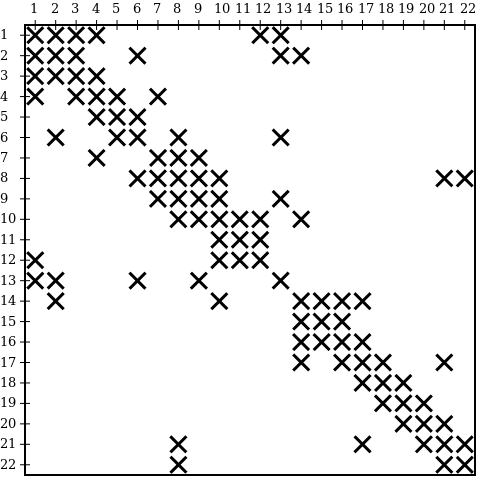
\includegraphics[width=0.3\textwidth]{mat}
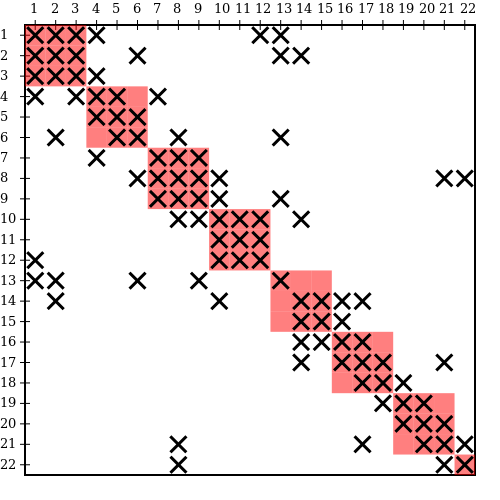
\includegraphics[width=0.3\textwidth]{mat_sparsify}
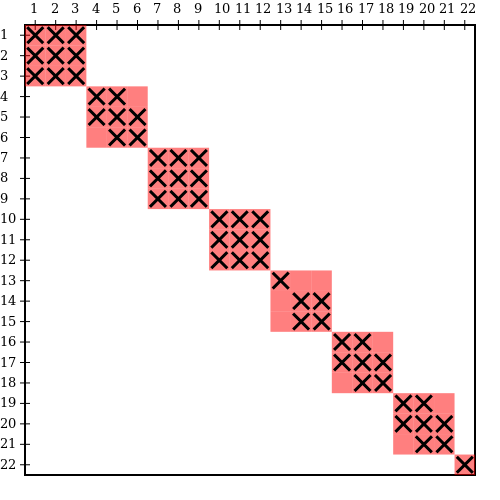
\includegraphics[width=0.3\textwidth]{mat_sparsify_removed}
\end{figure}
\end{frame}

\begin{frame}{Influence of Sparsification}
\begin{figure}
\centering
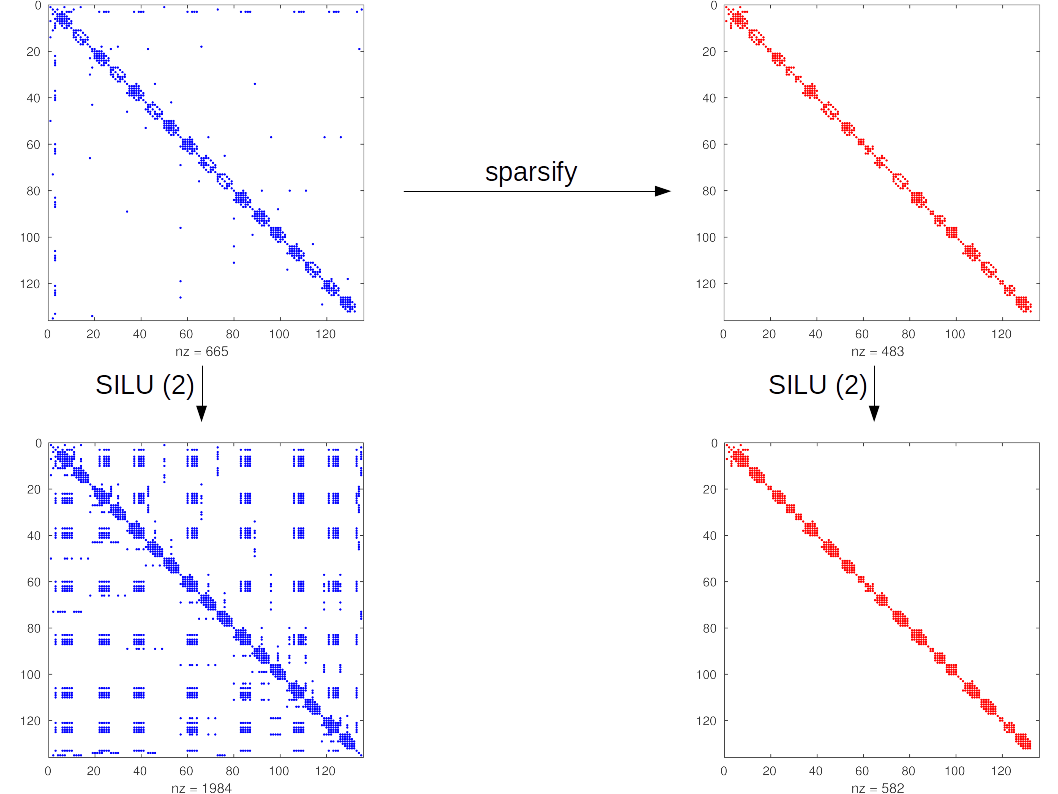
\includegraphics[width=0.8\textwidth]{sparsify}
\end{figure}
\end{frame}

\begin{frame}{AD, Preconditioning, and Sparsification}
\begin{itemize}
  \item To perform a Jacobian-vector product $J \vek{z}$ with some vector \vek{z} in a
      iterative solver method, apply automatic differentiation with a seed matrix
      identical to that vector \vek{z}. 
  \item Choose a block size $k$ and apply the sparsification to get \sparsify{J} from
      the Jacobian~$J$. Assemble \sparsify{J} via automatic differentiation and store
      it explicitly.
  \item Construct a preconditioner $M$ from \sparsify{J} by performing an ILU(0)
      factorization on each block of~\sparsify{J}. 
\end{itemize}
\end{frame}


\begin{frame}{Problem Formulation: Block Seed}
Let $J$ be a sparse $n \times n$ Jacobian matrix with known sparsity pattern and let
\sparsify{J} denote its sparsification using $k \times k$ blocks on the diagonal of $J$.
Find a binary $n \times p$ seed matrix~$S$ with a minimal number of columns, $p$, such
that all nonzero entries of \sparsify{J} also appear in the compressed matrix $J \cdot
S$.
\end{frame}

\begin{frame}{Full vs Partial Jacobian Computation}
%------------------------------------------------------------------------------------------
\begin{figure}
\centering
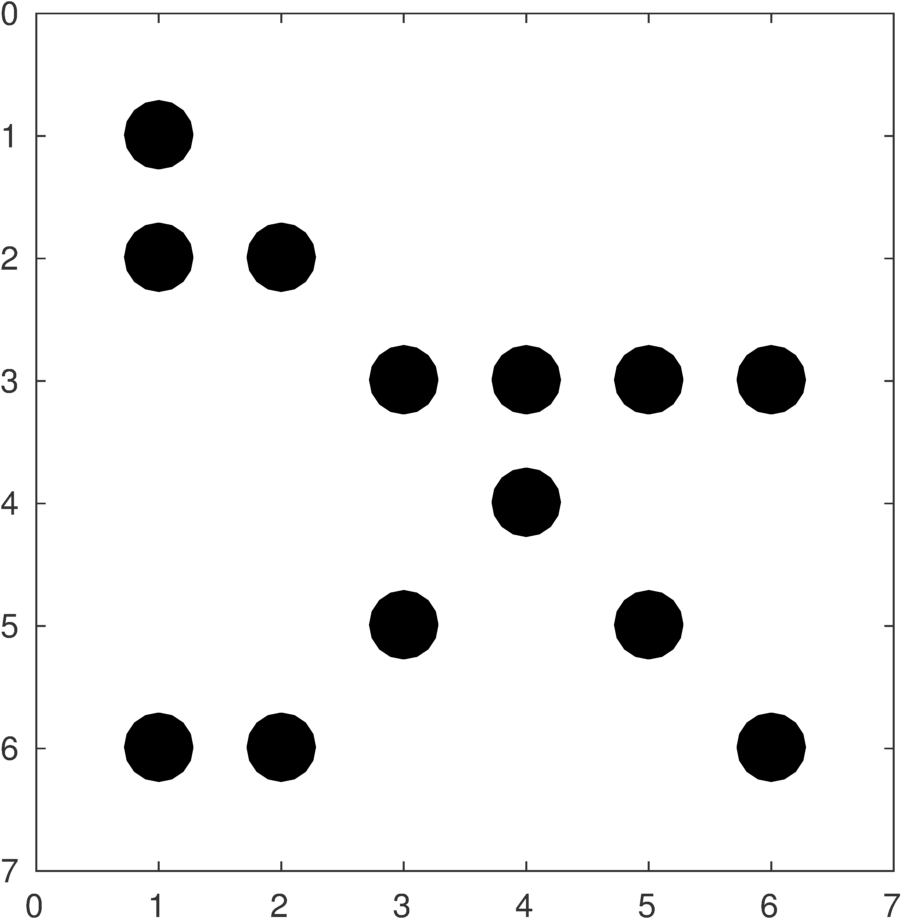
\includegraphics[height=0.25\textwidth]{small_jac}
\hfill
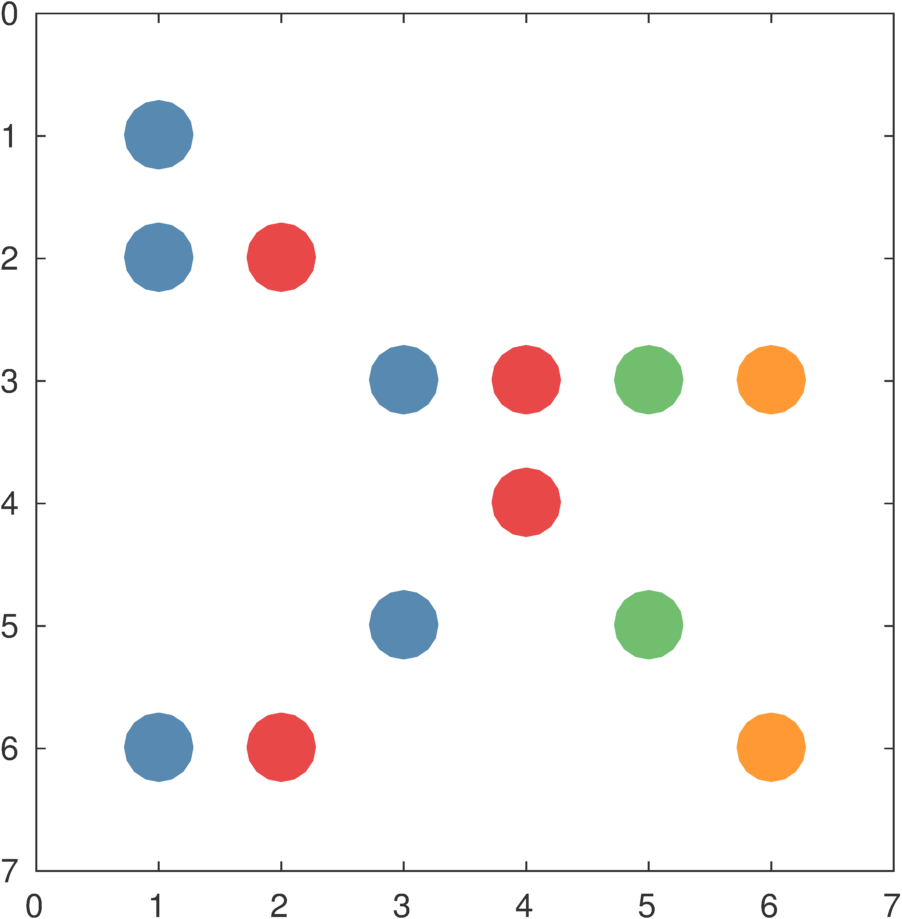
\includegraphics[height=0.25\textwidth]{full_color}
\hfill
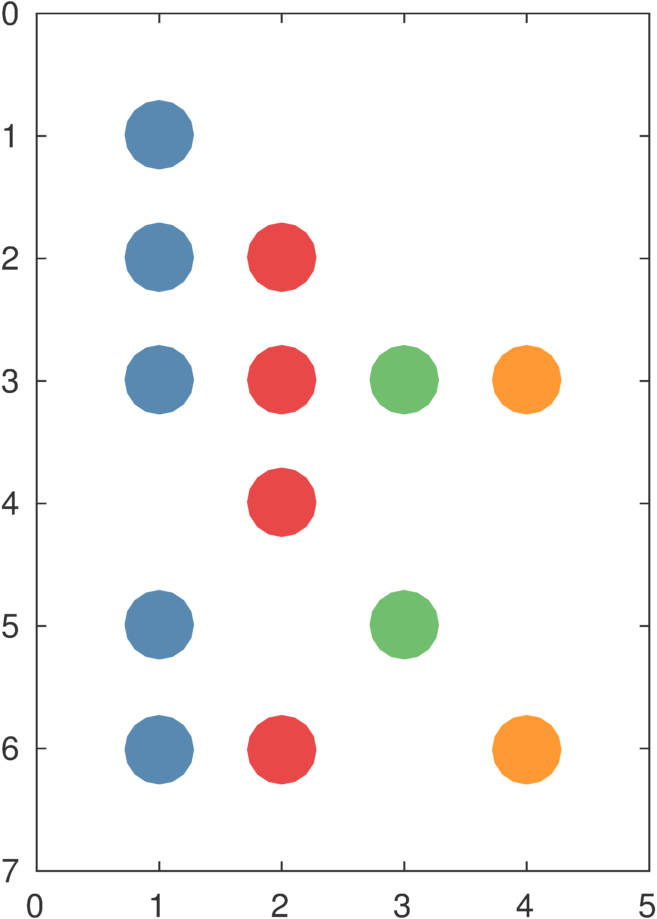
\includegraphics[height=0.25\textwidth]{full_color_compress}
\end{figure}
\noindent\makebox[\linewidth]{\rule{\paperwidth}{0.4pt}}
\begin{figure}
\centering
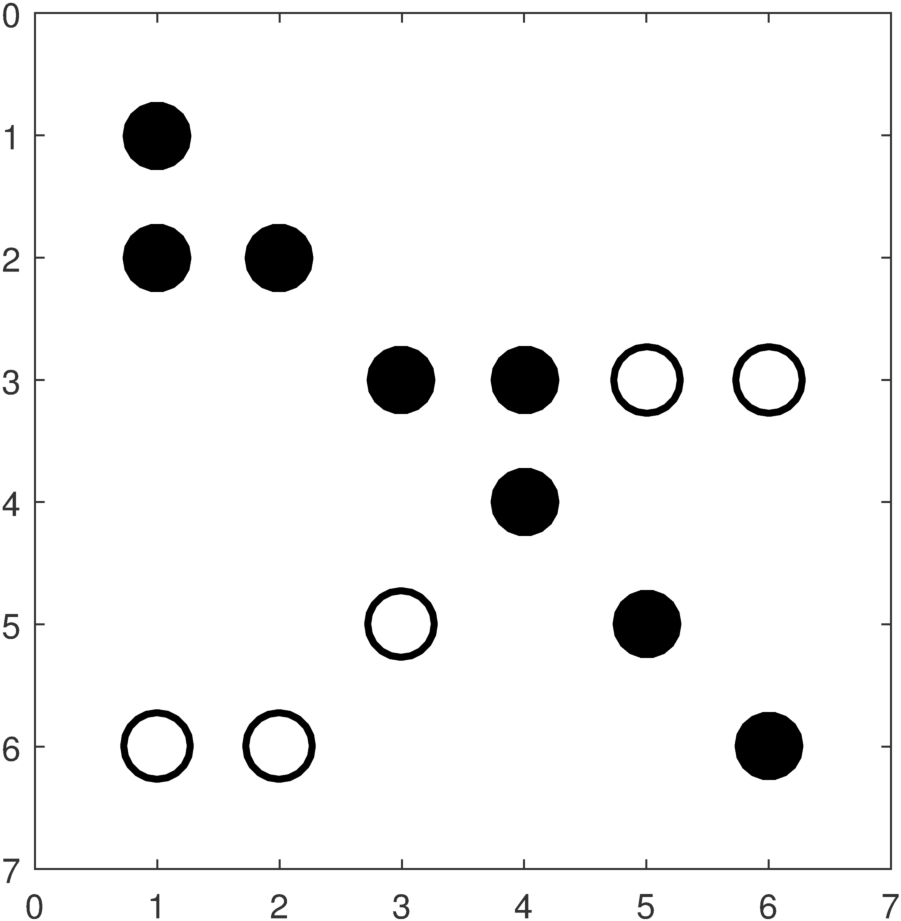
\includegraphics[height=0.25\textwidth]{partial_coloring_orig}
\hfill
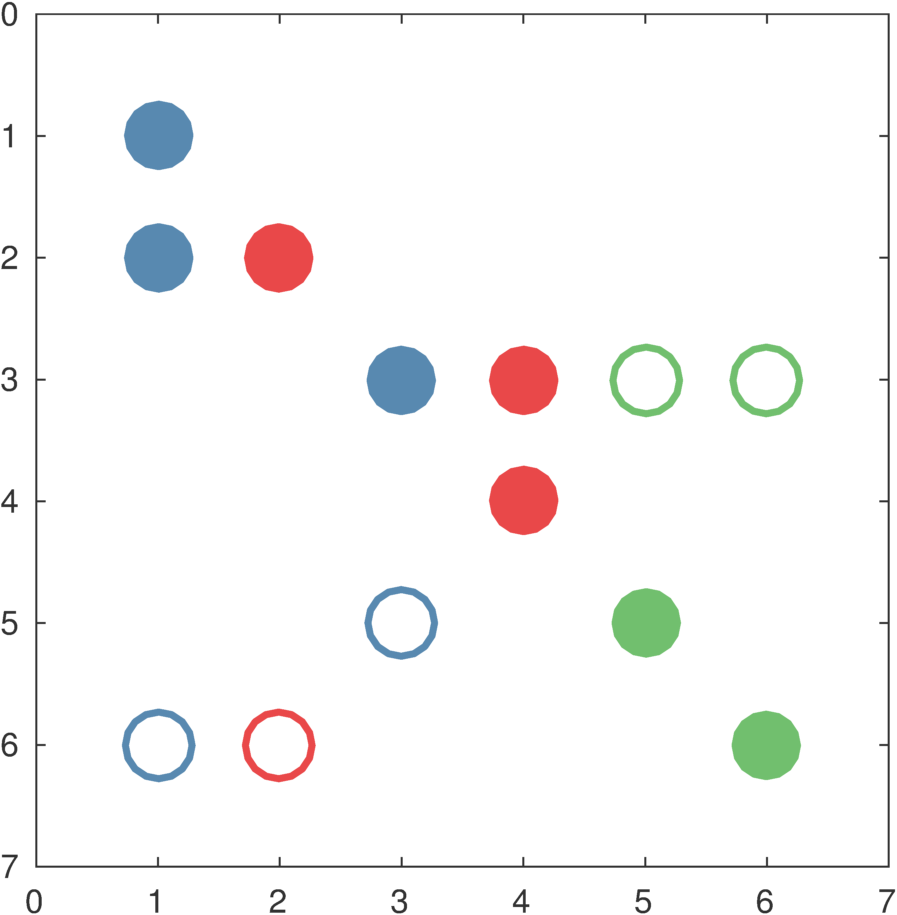
\includegraphics[height=0.25\textwidth]{partial_color}
\hfill
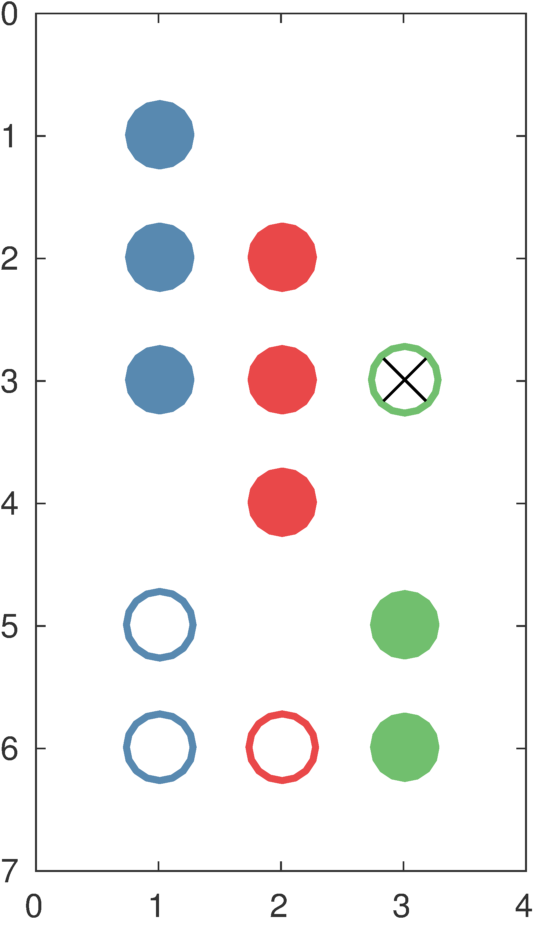
\includegraphics[height=0.25\textwidth]{partial_color_compress}
\end{figure}
%------------------------------------------------------------------------------------------

\end{frame}


\begin{frame}{Combinatorial Model: Bipartite Graph}
$G(V_c\times V_r,E)$
\begin{figure}
\centering
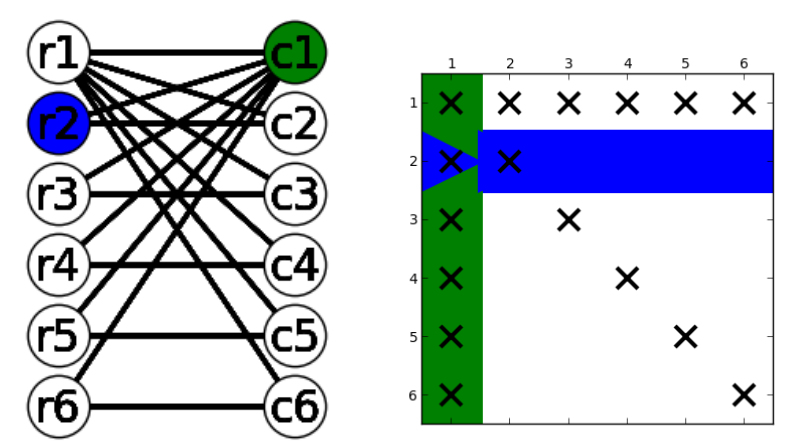
\includegraphics[width=0.8\textwidth]{bip}
\end{figure}
\end{frame}

\begin{frame}{Restrticted Distnace-$2$ Coloring}
Given the bipartite graph $G(V_c\times V_r,E)$ and the required elements
$E_D$, the distance-$2$ coloring restricted to $E_D$ is the mapping 
$\Phi:V_c\to {0,1,...,p}$ such that
\begin{itemize}
\item $\forall (r_i,c_i)\in E_D:\Phi(c_i)\neq 0$
\item The distance-$2$ neighbors $c_i, c_j$ are colored differently
if there is a connecting path of length $2$ with at least an edge in $E_D$.
\end{itemize}
\begin{figure}
\centering
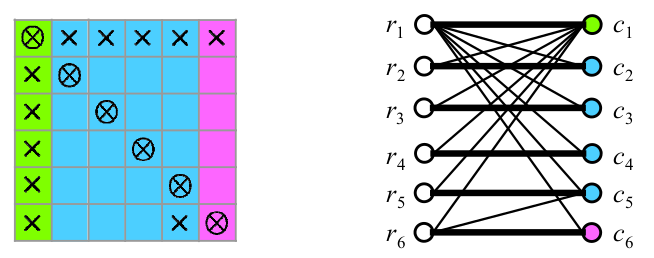
\includegraphics[width=0.8\textwidth]{restricted_distance2}
\end{figure}
\end{frame}

\begin{frame}{Different Models of Computation}
\begin{figure}
\centering
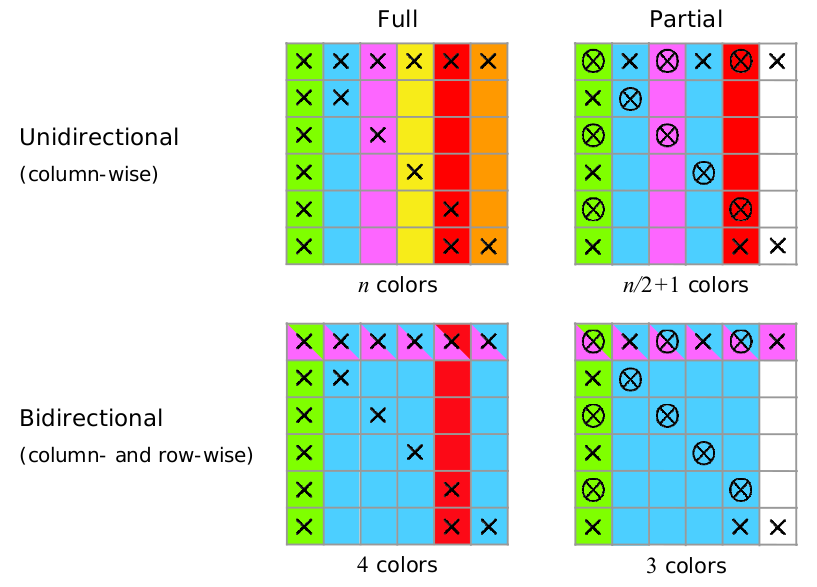
\includegraphics[width=0.9\textwidth]{fullvsPart}
\end{figure}
\end{frame}

\begin{frame}{Combining AD and Preconditioning}
\begin{figure}
\centering
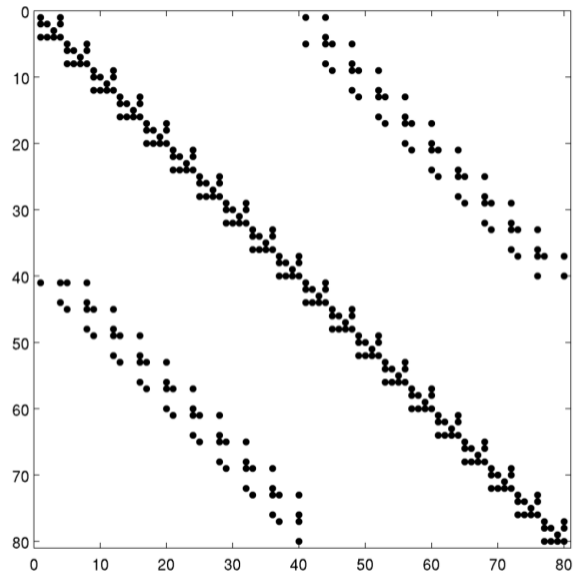
\includegraphics[width=0.29\textwidth]{nnz}
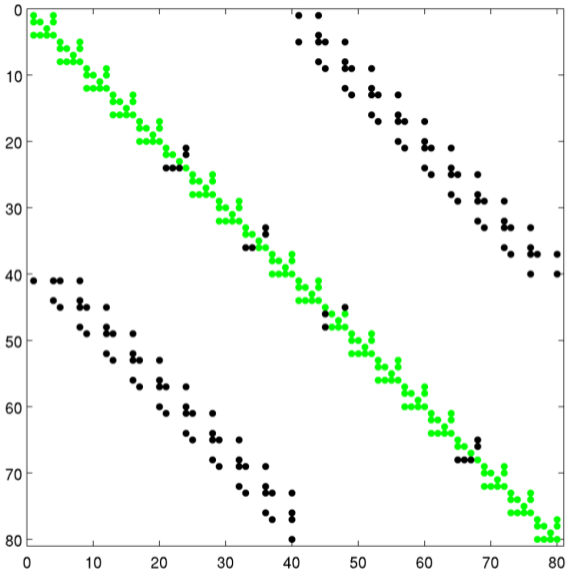
\includegraphics[width=0.29\textwidth]{nnz_Ri}
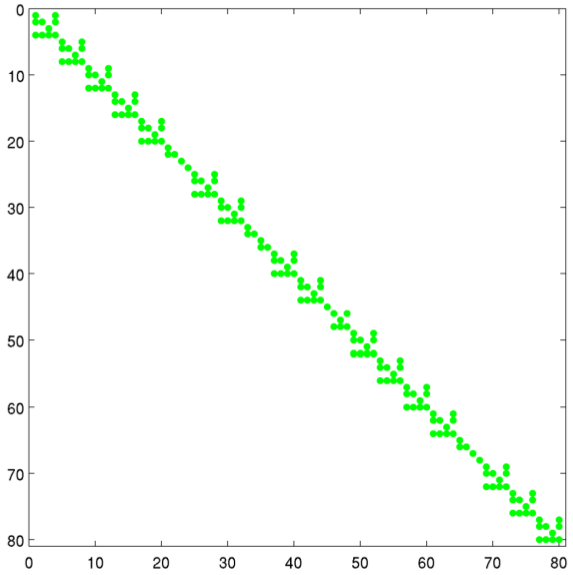
\includegraphics[width=0.29\textwidth]{R_i}
\end{figure}
\begin{figure}
\centering
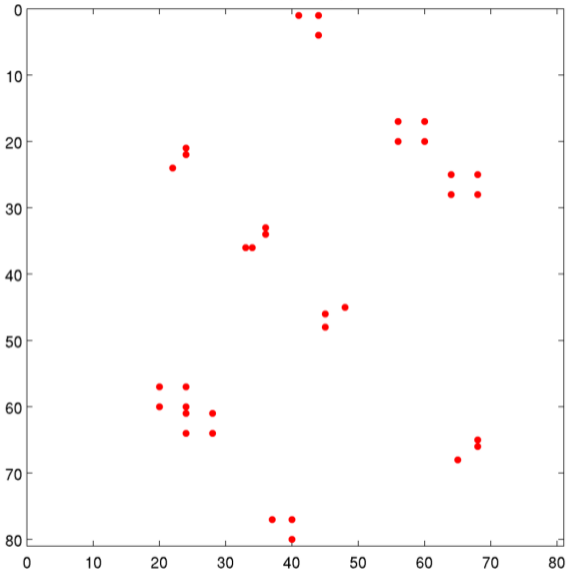
\includegraphics[width=0.29\textwidth]{P}
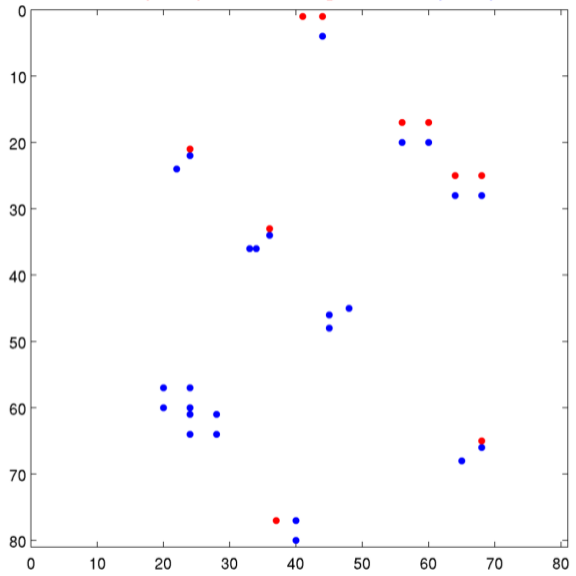
\includegraphics[width=0.29\textwidth]{PA}
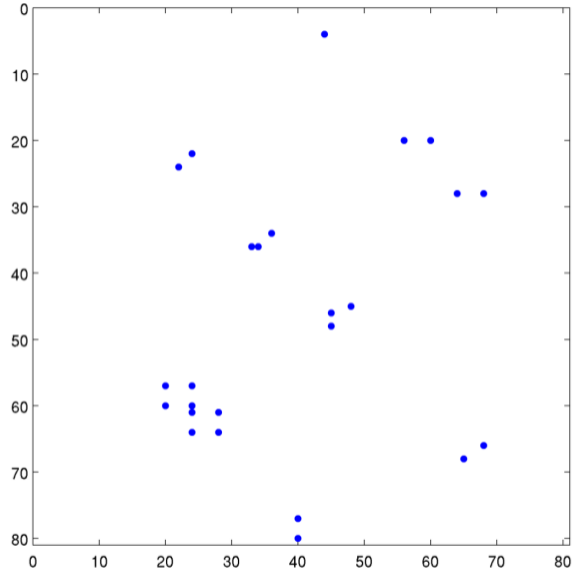
\includegraphics[width=0.29\textwidth]{add}
\end{figure}
\end{frame}

\section{New Coloring Heuristics}
\begin{frame}{Increasing the potentially and additionally required elements}
The nonrequired nonzero elements are also computed as a by-product of the computation of required elements.
The nonrequired elements have a major effect on the determination of potentially required elements
and additionally required elements.
\begin{figure}
\centering
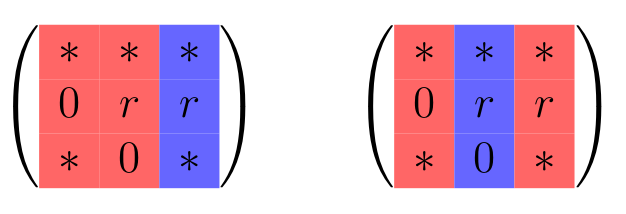
\includegraphics[width=0.5\textwidth]{increase}
\end{figure}
\end{frame}

\begin{frame}[fragile]
\frametitle{Restricted Distance-$2$ Coloring Heuristics}
The greedy algorithm for
the distance-$2$ coloring restricted to the edge set $E_i$
for columns.
\begin{lstlisting}[mathescape]
function d2_color($G=(V_r\cup V_c,E)$,$E_i\subseteq E$)
  $\Phi\leftarrow [0\ldots 0]$
  $forbiddenColors\leftarrow [0\ldots 0]$
  for $v\in V_c$ with $\exists r\in V_r: (v,r) \in E_i$
    for $n\in N_2(v,E_i)$ with $\Phi(n) \neq 0$
        $forbiddenColors[\Phi(n)] = v$
    $\Phi(v) = \min \{ a>0:forbiddenColors[a]\neq v\}$
  return $\Phi$
\end{lstlisting}
\end{frame}
\begin{frame}[fragile]
\frametitle{New coloring heuristic}
New coloring heuristic for distance-$2$ coloring
considering the nonrequired elements.
\begin{figure}
\begin{lstlisting}[mathescape]
function d2_color_nreq($G=(V_r\cup V_c,E)$,$E_i\subseteq E$)
  $\Phi\leftarrow [0\ldots 0]$
  $forbiddenColors\leftarrow [0\ldots 0]$
  for $v\in V_c$ with $\exists r\in V_r: (v,r) \in E_i$ and $\Phi(v)=0$
    for $n\in N_2(v,E_i)$ with $\Phi(n) \neq 0$
      $forbiddenColors[\Phi(n)] = v$
    $\Phi(v) = \min \{ a>0:forbiddenColors[a]\neq v\}$

    $I_v=\{z\in V_c: z\neq v\text{ and }z\notin N_2(v) \text{ and } \Phi(z) = 0 \}$
    if $I_v\neq\emptyset$
      $maxs = \argmax_{x\in I_v} \nreq_v (x)$
      $\Phi(maxs[0]) = \Phi(v)$
  return $\Phi$
\end{lstlisting}
\end{figure}
\end{frame}

\begin{frame}{Results}
\begin{table}
\begin{center}
\begin{tabular}{|c|c|c|c|c|}
\hline
Matrix (NAT) & \multicolumn{2}{c|}{$|R_p|$} & \multicolumn{2}{c|}{$|R_a|$}\\\hline
{} & Greedy & New & Greedy & New\\\hline
\textit{steam1.mtx} & $64$ & $786$ & $64$ & $630$ \\\hline
\textit{steam2.mtx} & $240$ & $1880$ & $240$ & $1400$ \\\hline
\textit{nos3.mtx} & $1638$ & $6756$ & $1106$ & $4296$ \\\hline
\textit{crystm01.mtx} & $17822$ & $47556$ & $10388$ & $28318$ \\\hline
\textit{ex7.mtx} & $38554$ & $34954$ & $29174$ & $25054$ \\\hline
\textit{ex33.mtx} & $7408$ & $8934$ & $4920$ & $5572$ \\\hline
\textit{coater1.mtx} & $11722$ & $11558$ & $7684$ & $7448$ \\\hline
\textit{pesa.mtx} & $36972$ & $41154$ & $31010$ & $33094$ \\\hline
\end{tabular}
\end{center}
\end{table}
\end{frame}

\begin{frame}{Comparing with different block sizes}
\begin{figure}
\centering
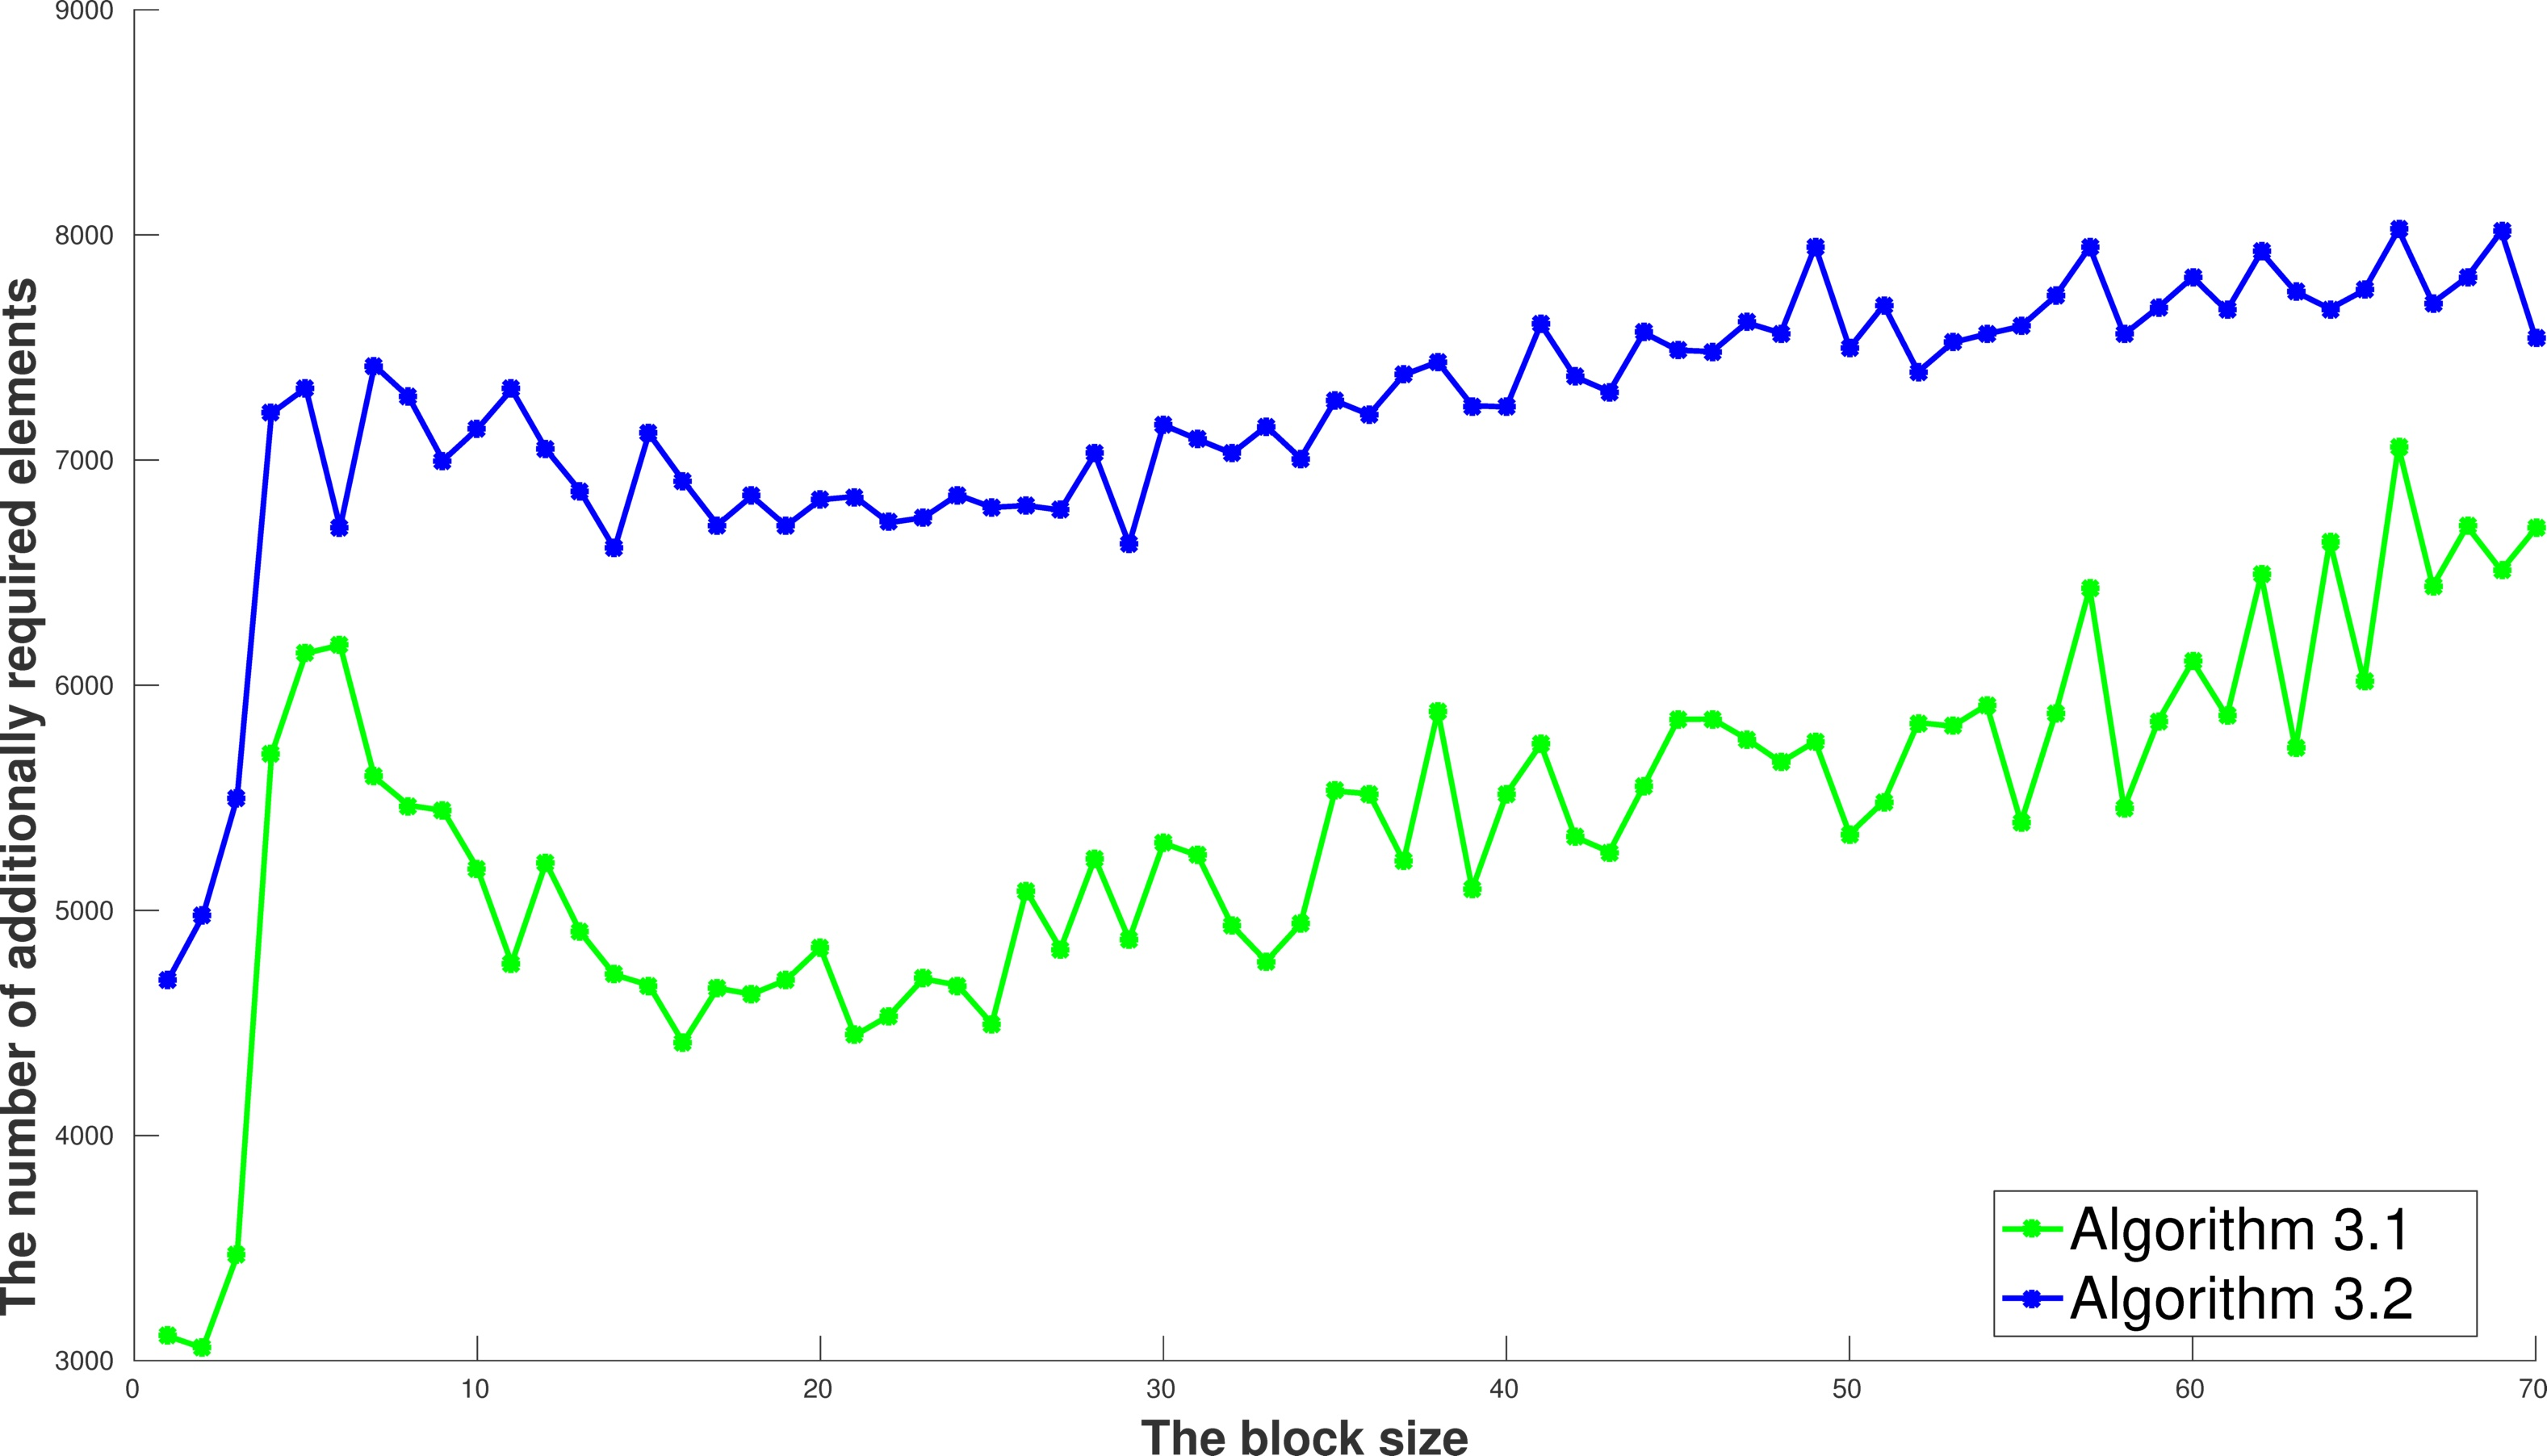
\includegraphics[width=0.9\linewidth]{ex33_alg31_alg32_bls_slo_add}
\caption{
The number of additionally required elements computed by
new heuristic with the SLO ordering
compared with Greedy algorithm.
The computation is carried out on the matrix \textit{ex33}. }
\label{ex33_alg31_alg32_bls_slo_add}
\end{figure}
\end{frame}

\begin{frame}[fragile]
\frametitle{Balancing the number of colors}
\begin{figure}
\begin{lstlisting}[
caption=New coloring heuristic with a controller to balance
the number of colors and the number of additionally required elements.,
label=code.new.impr2,mathescape]
function d2_color_nreq_balance($G=(V_r\cup V_c,E)$,$E_i\subseteq E$,$\alpha$)
  $\Phi\leftarrow [0\ldots 0]$
  $forbiddenColors\leftarrow [0\ldots 0]$
  for $v\in V_c$ with $\exists r\in V_r: (v,r) \in E_i$ and $\Phi(v)=0$
    for $n\in N_2(v,E_i)$ with $\Phi(n) \neq 0$
      $forbiddenColors[\Phi(n)] = v$
    $\Phi(v) = \min \{ a>0:forbiddenColors[a]\neq v\}$

    $I_v=\{z\in V_c: z\neq v\text{ and }z\notin N_2(v) \text{ and } \Phi(z) = 0 \}$
    if $I_v\neq\emptyset$
      $maxs = \argmax_{x\in I_v} \nreq_v (x)$
      $mins = \argmin_{x\in maxs} \req(x)$
      for $i\in\{0,1,...,\min (\alpha - 1, \operatorname{size}(mins)-1)\}$
        $\Phi(mins[i]) = \Phi(v)$
  return $\Phi$
\end{lstlisting}
\end{figure}
\end{frame}

\begin{frame}{Colors and number of additionally required elements}
\begin{figure}
\centering
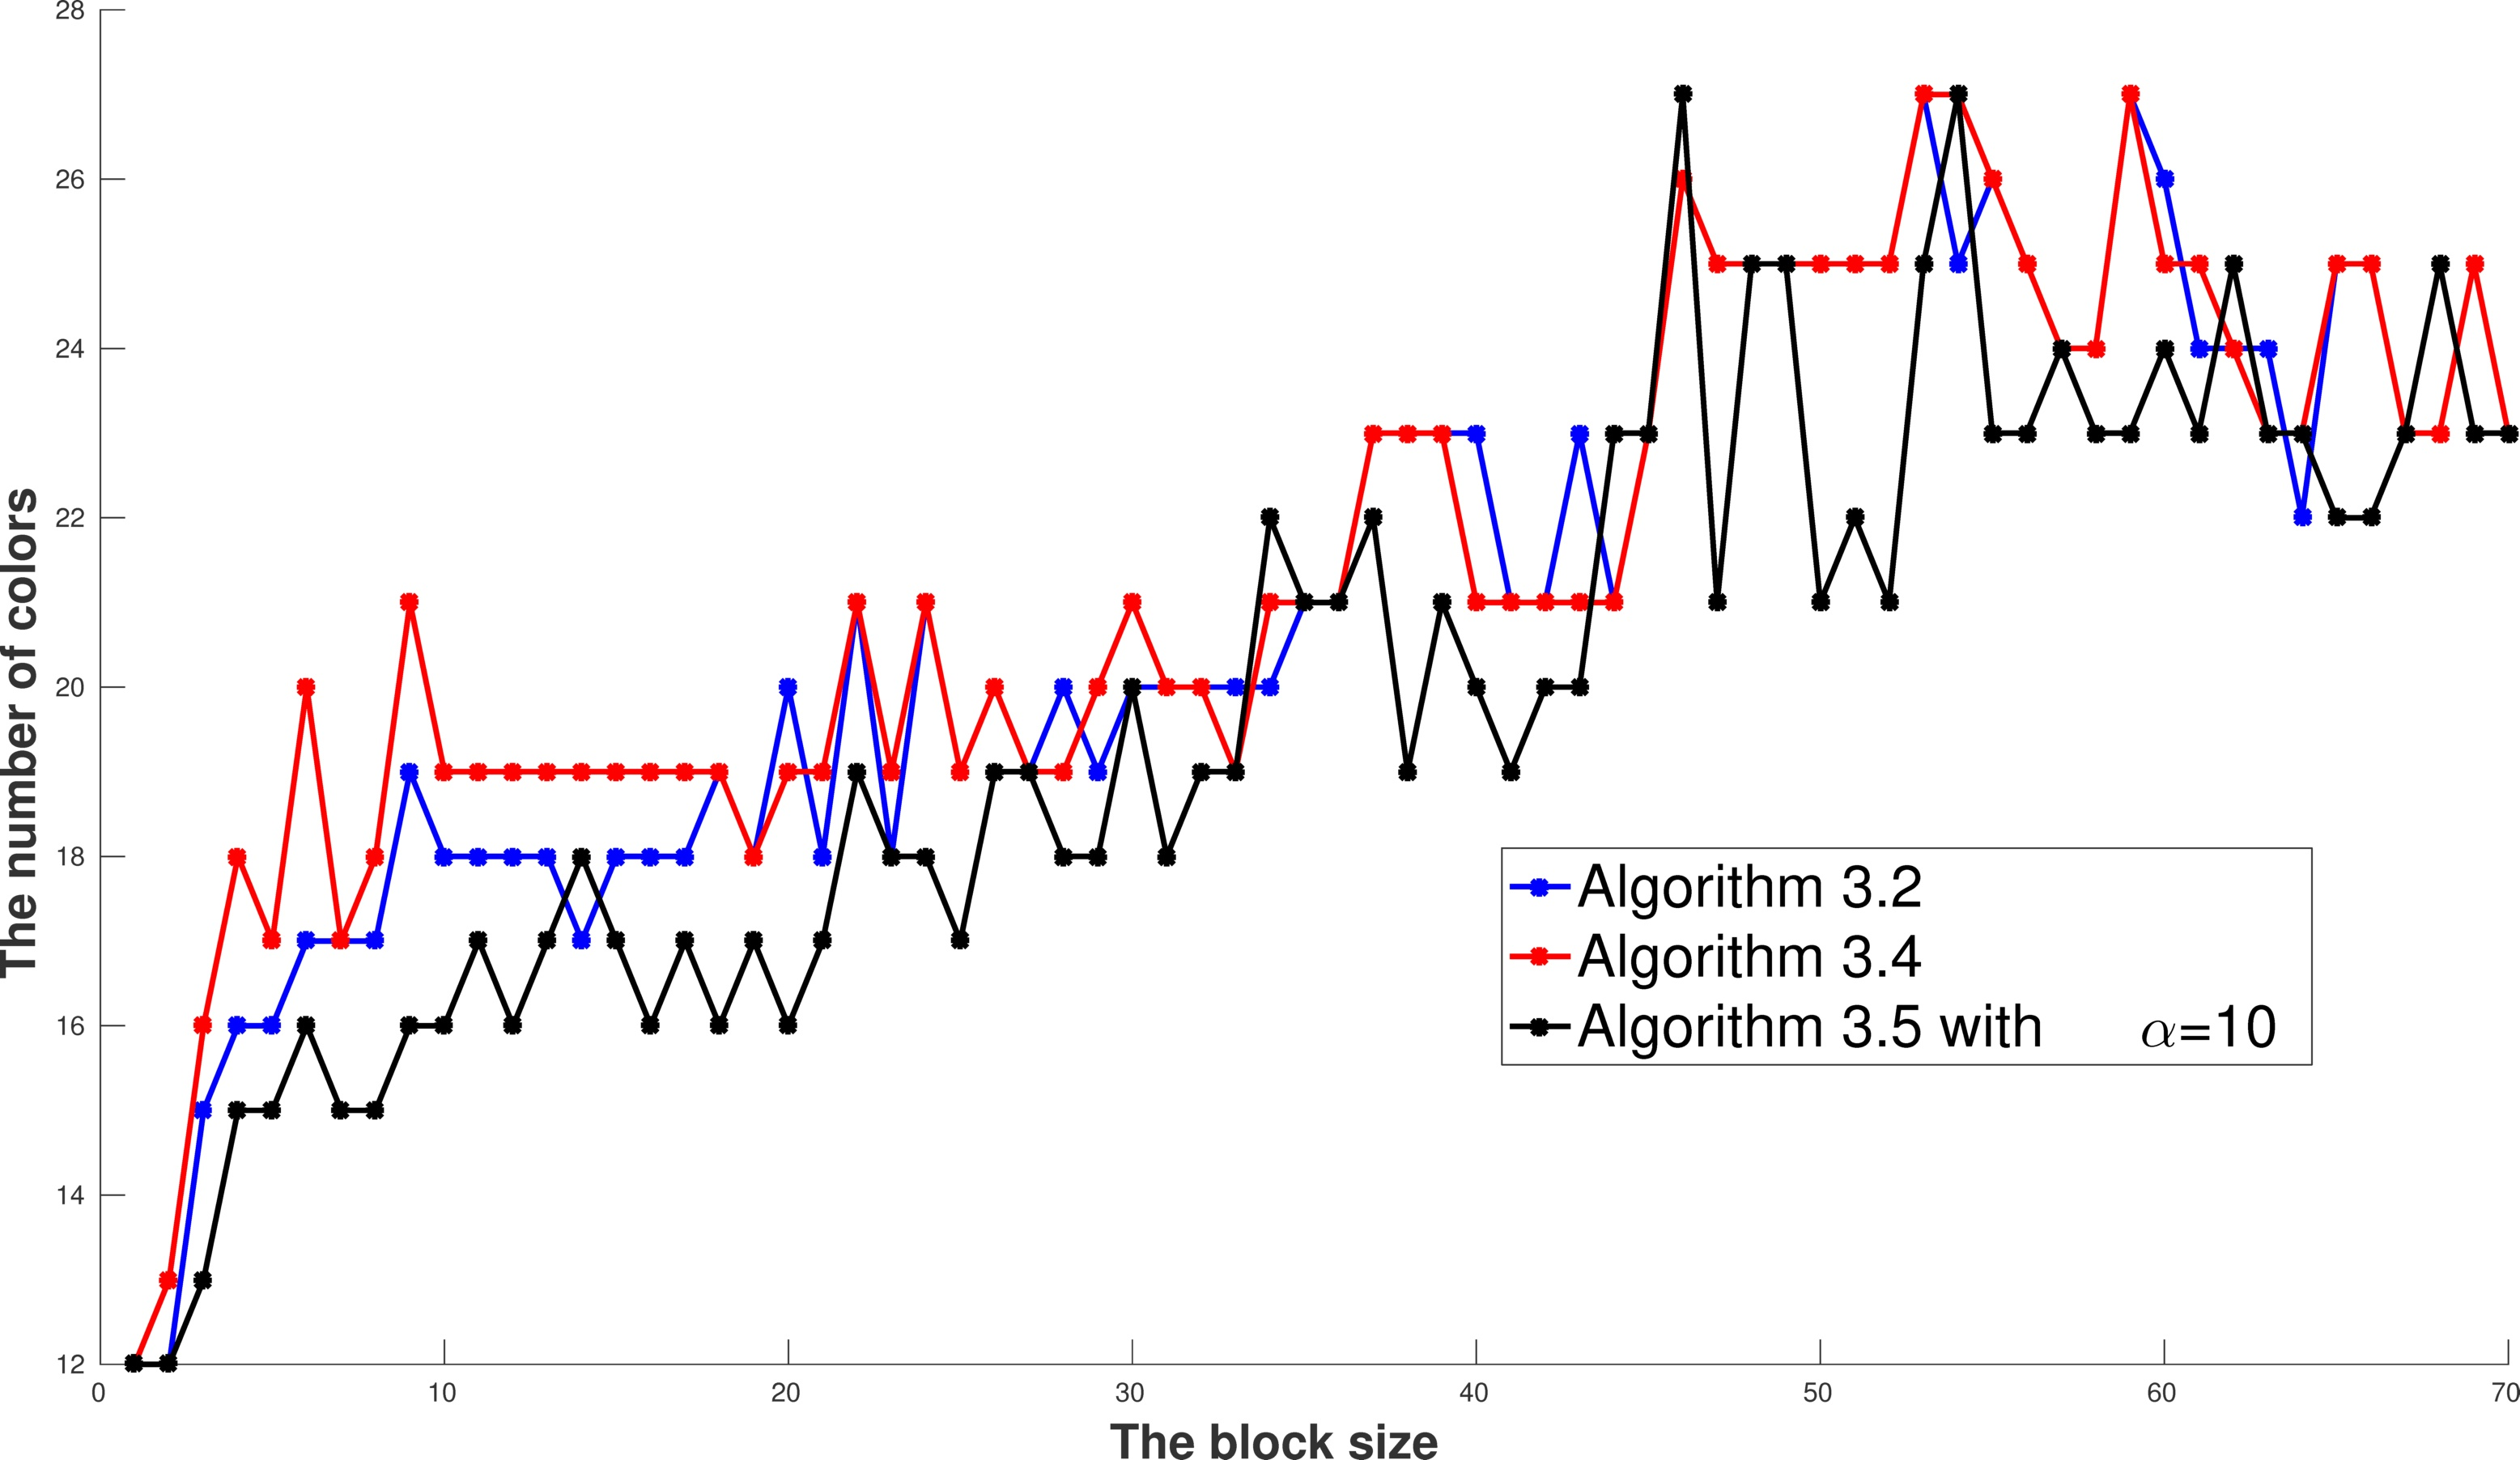
\includegraphics[width=0.5\linewidth]{ex33_alg31_alg32_alg34_alg35_bls_lfo_cols}
%The comparison of the number of colors in \coderef{code.new.d2.nreq},
%\coderef{code.new.impr1}, and~\coderef{code.new.impr2}.
%The computation is carried out on the matrix \textit{ex33} and with the LFO ordering.}
\label{ex33_alg31_alg32_alg34_alg35_bls_lfo_cols}
\end{figure}

\begin{figure}
\centering
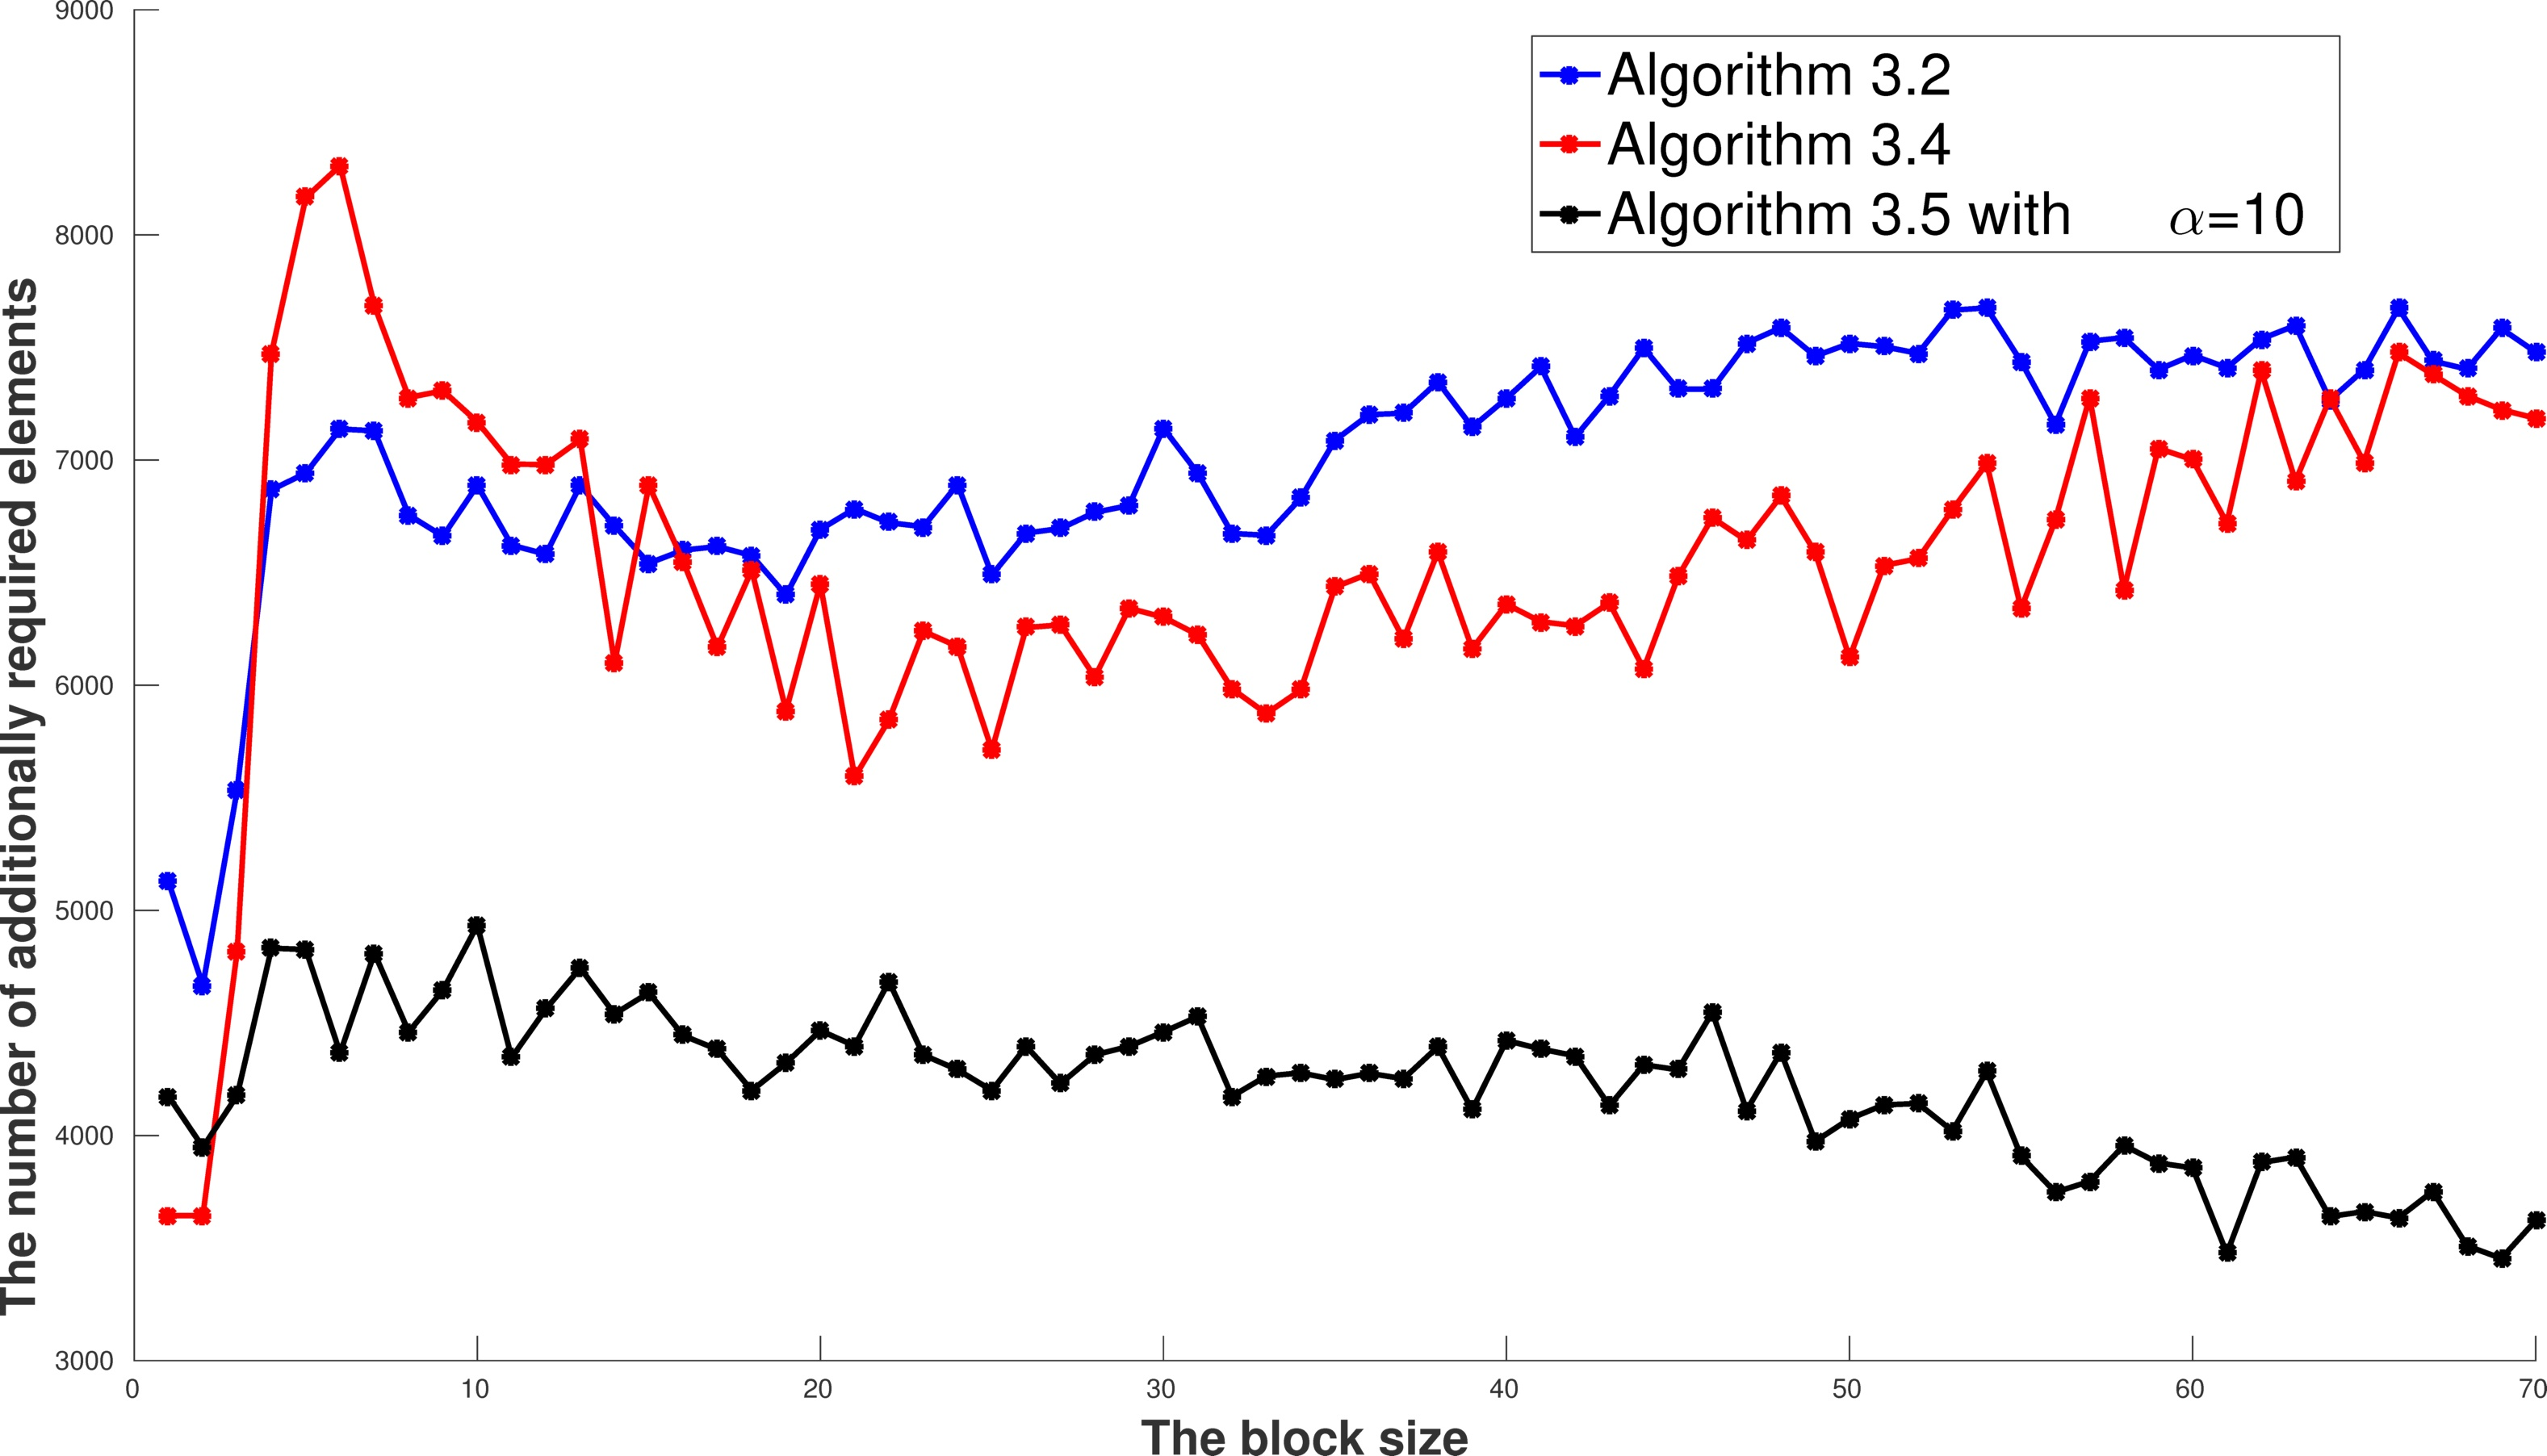
\includegraphics[width=0.5\linewidth]{ex33_alg31_alg32_alg34_alg35_bls_lfo_adds}
%The comparison of the number of additionally required elements in \coderef{code.new.d2.nreq},
%\coderef{code.new.impr1}, and~\coderef{code.new.impr2}.
%The computation is carried out on the matrix \textit{ex33} and with the LFO ordering.}
\label{ex33_alg31_alg32_alg34_alg35_bls_lfo_adds}
\end{figure}
\end{frame}

\section{Application}
\begin{frame}{Application in Geoscience}
we apply our new heuristics to a carbon sequestration example from geoscience.
The geophysics group of RWTH Aachen simulates the injection of CO$_2$ in a reservoir by a
two-phase flow model in porous media.
\begin{figure}
\centering
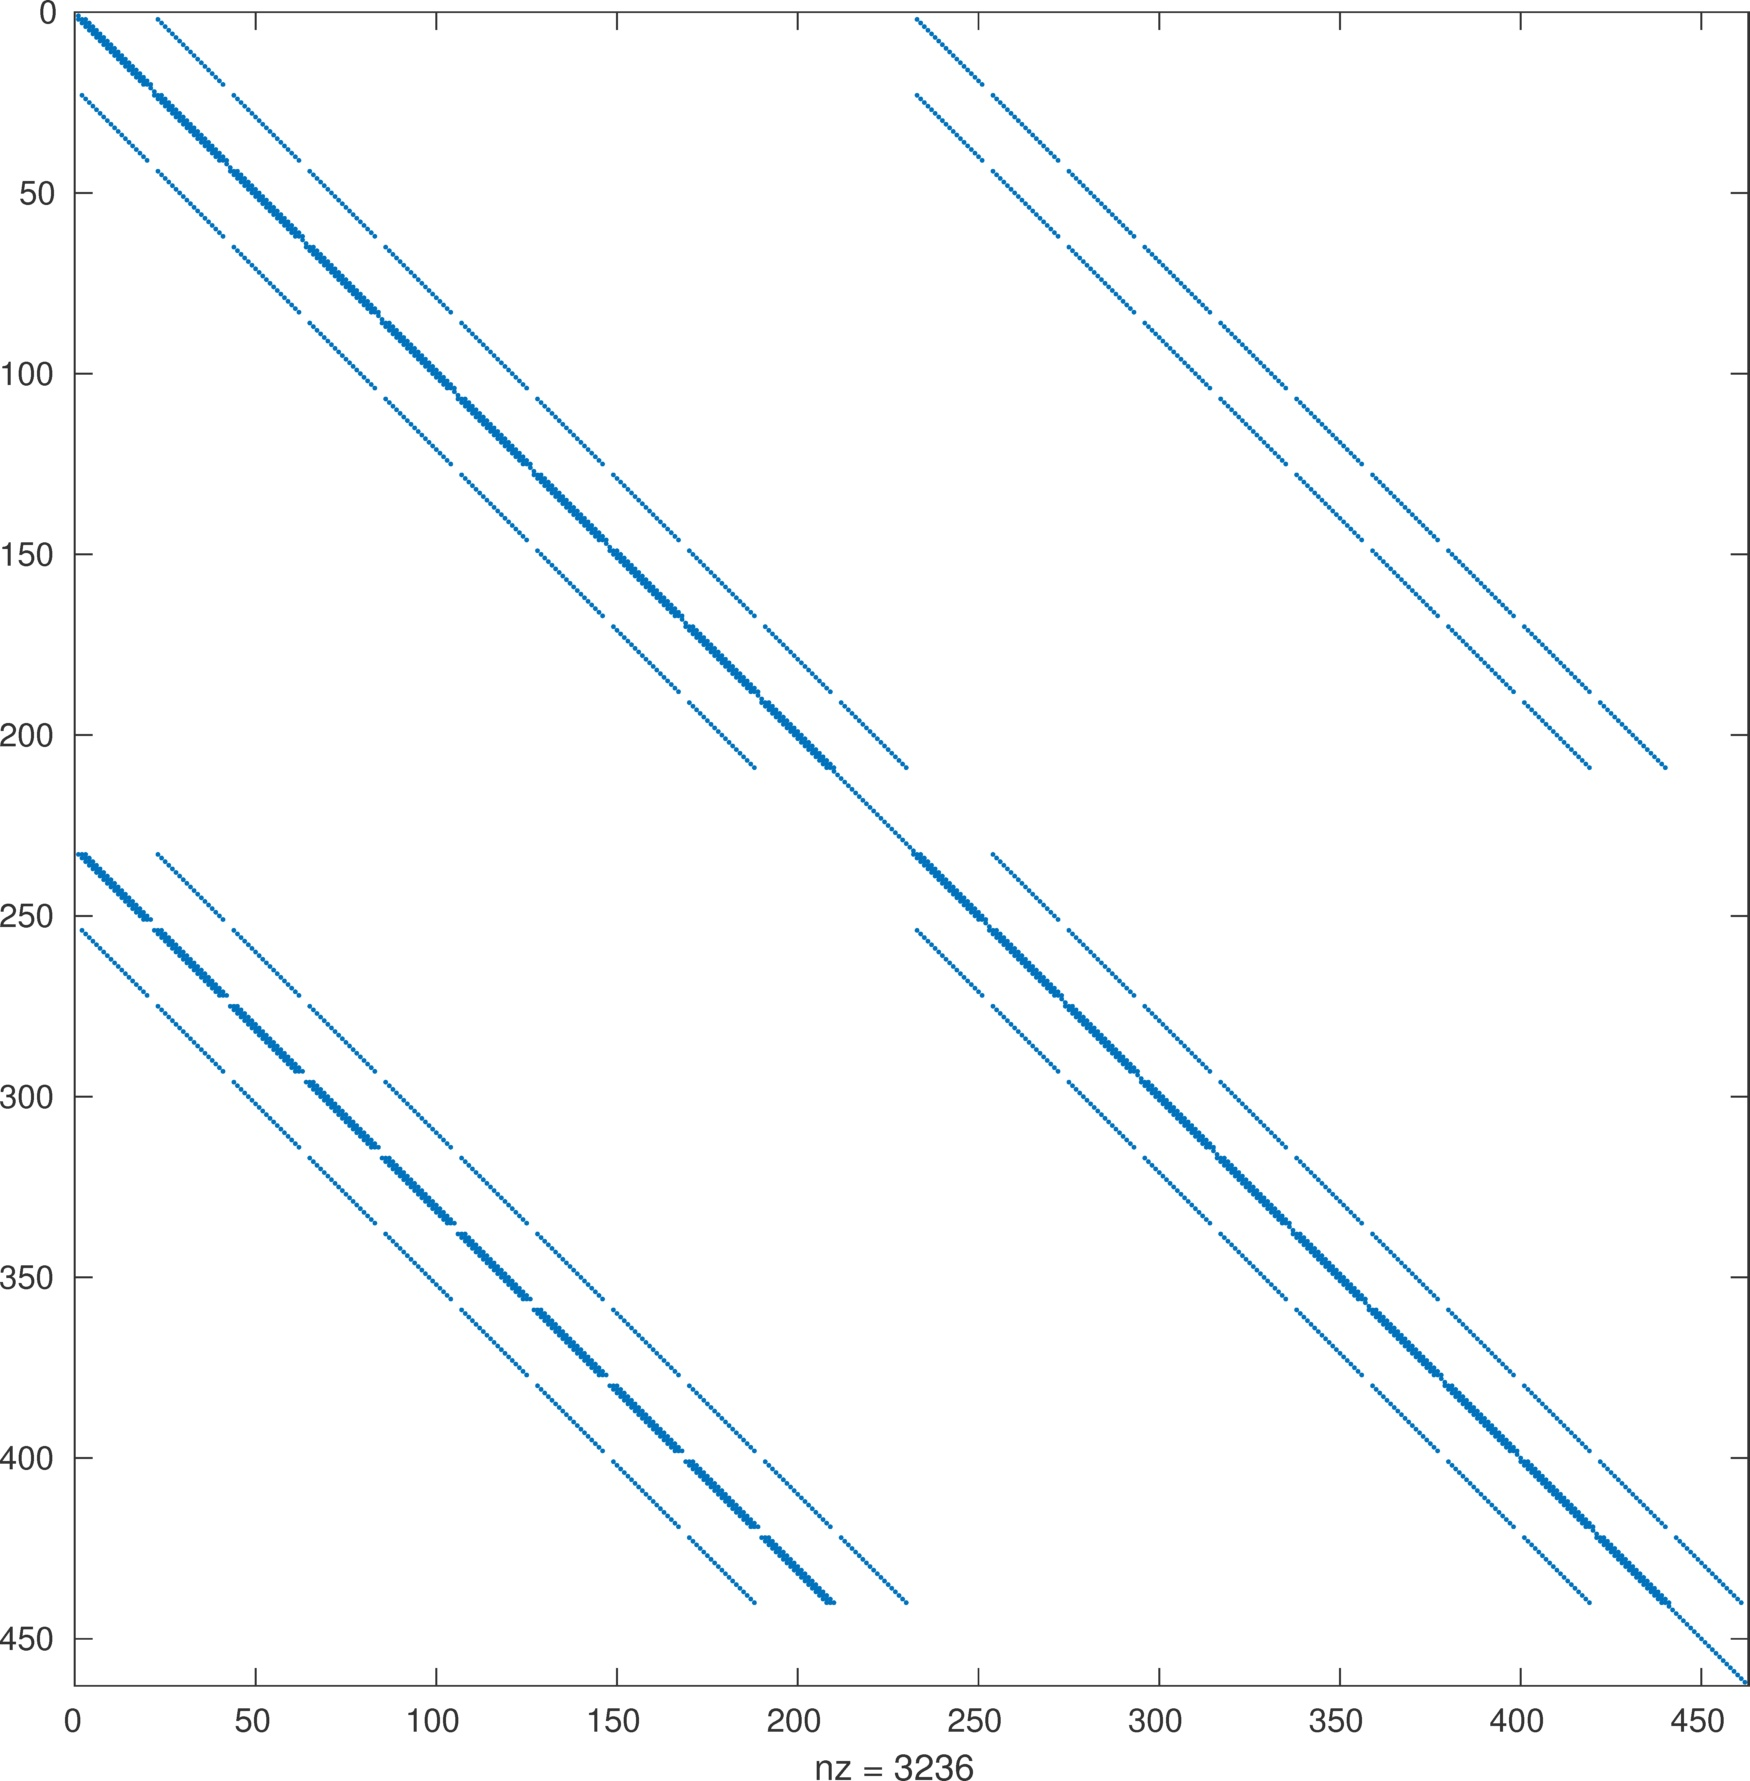
\includegraphics[width=0.4\textwidth]{co2_jac}
\end{figure}
\end{frame}

\begin{frame}{Convergence (Block Size = 5)}
\begin{figure}
\centering
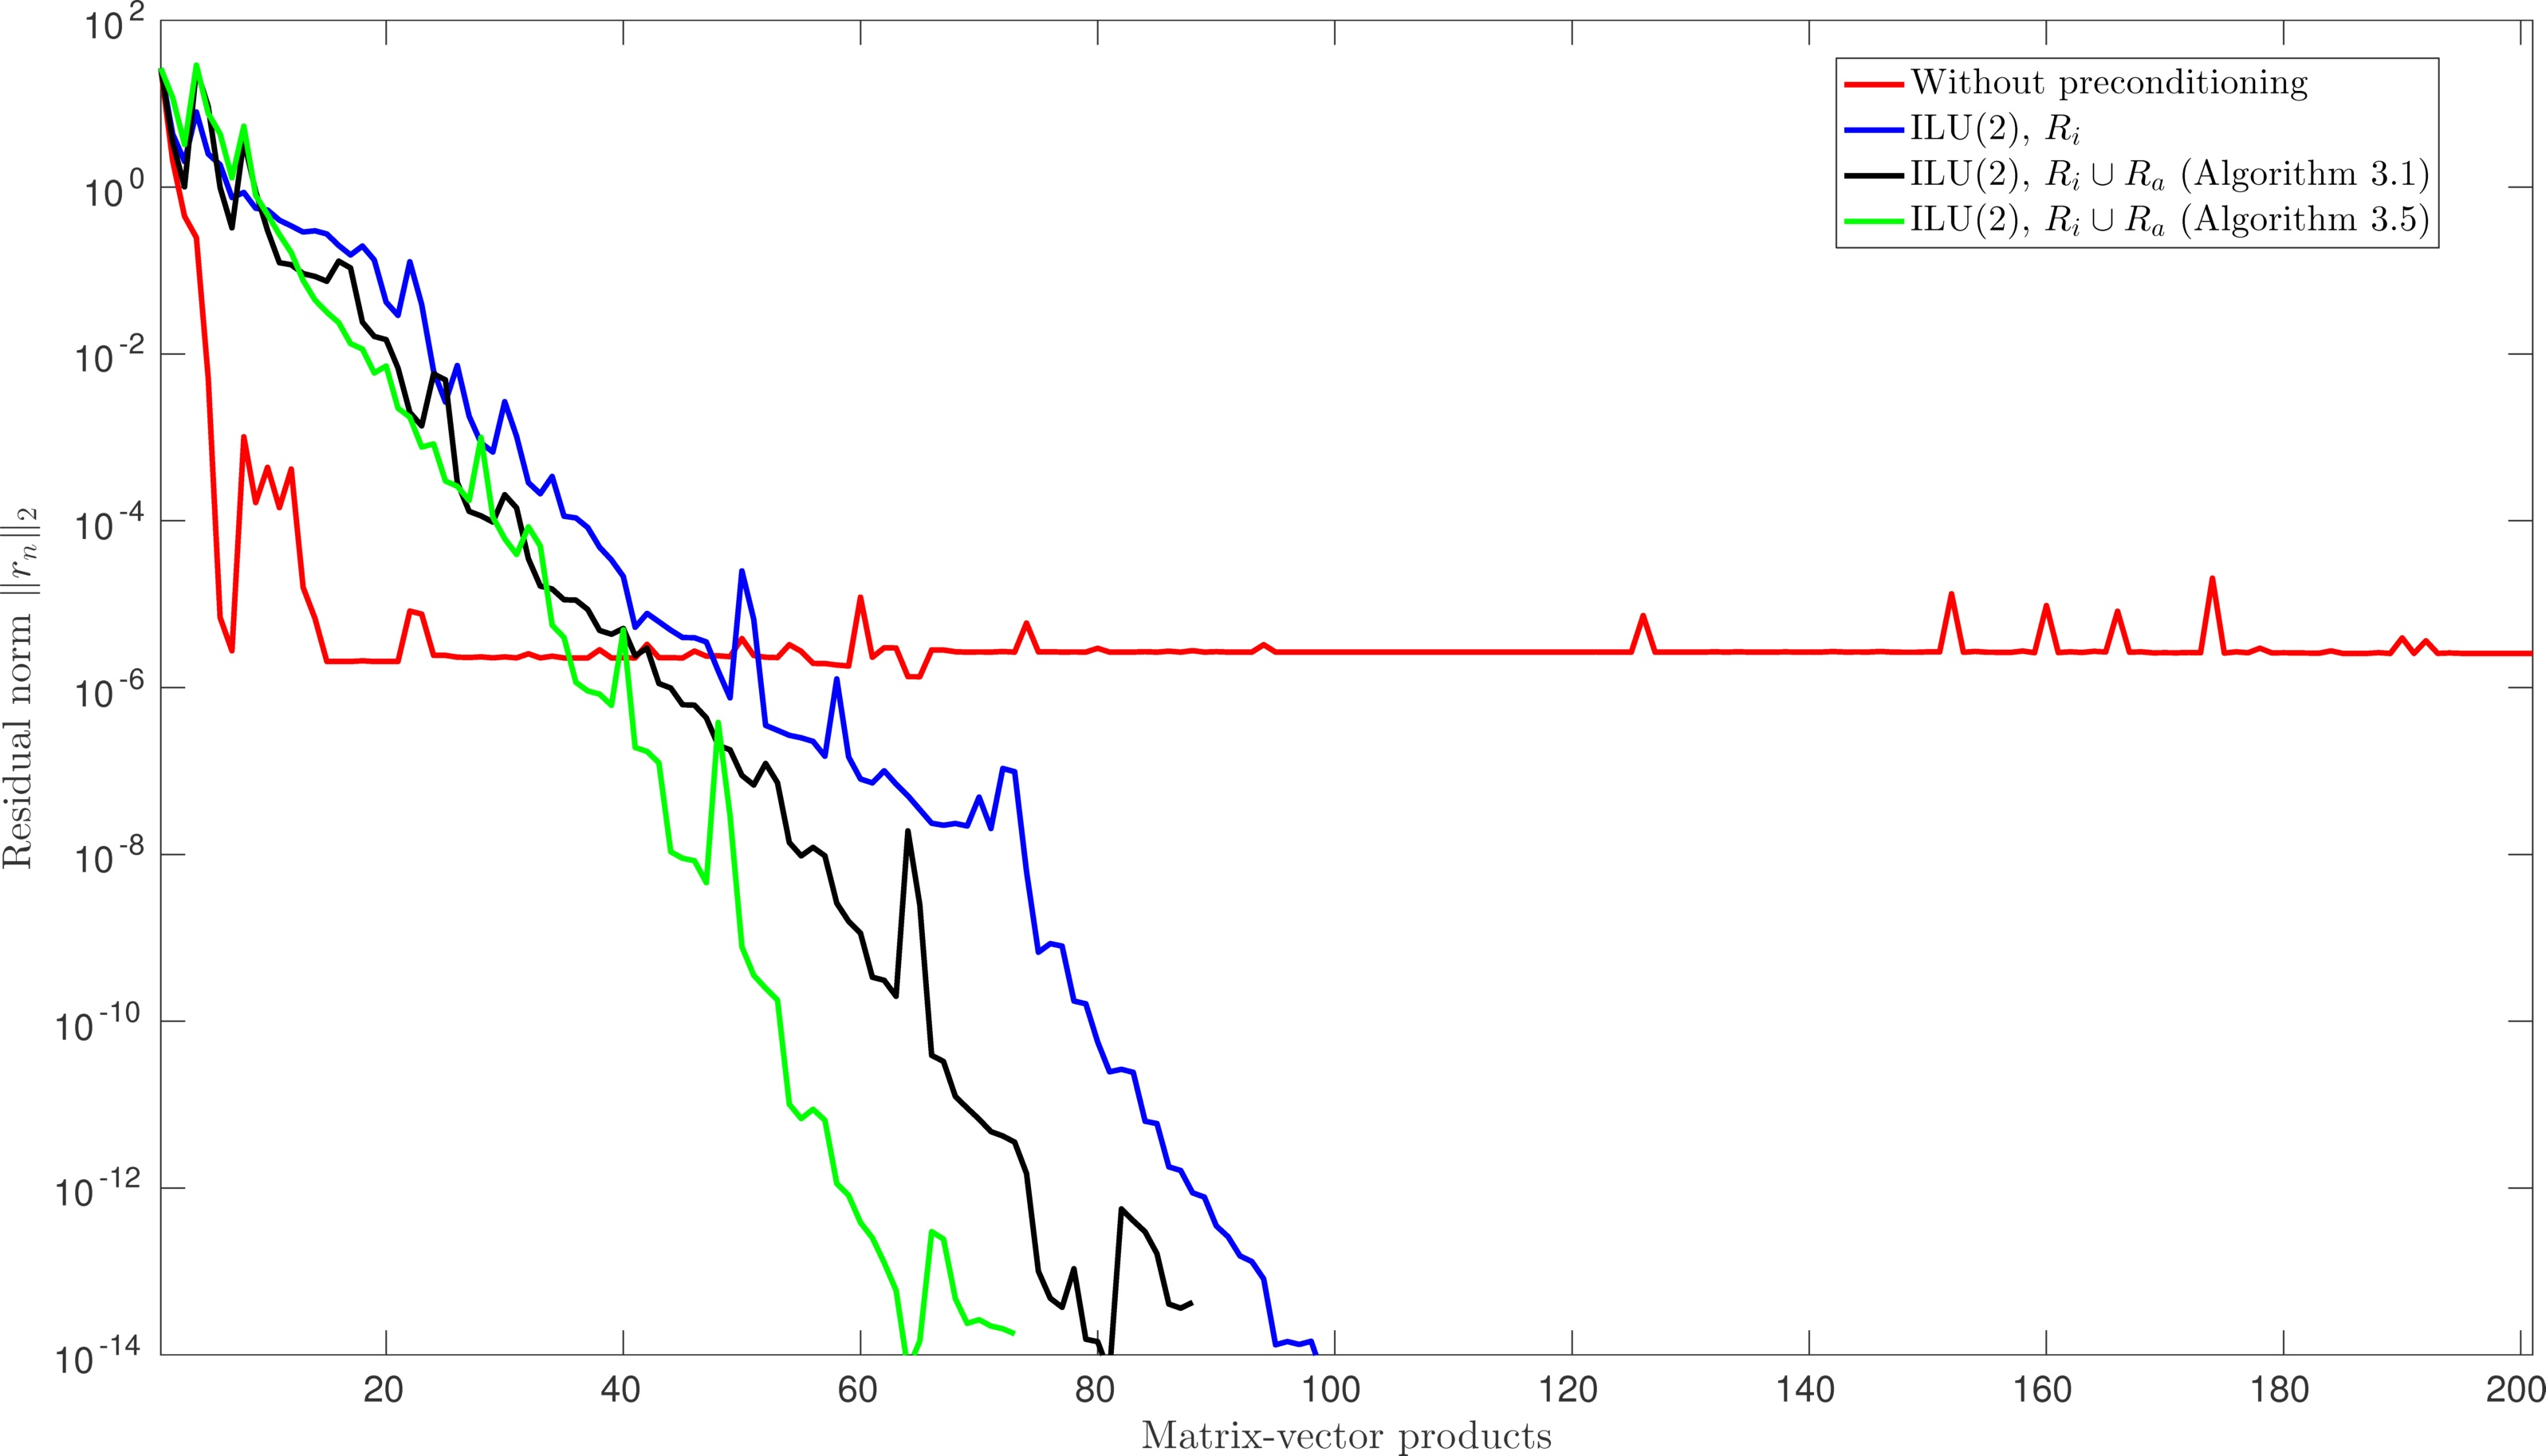
\includegraphics[width=0.9\textwidth]{jac_convergence_greedy_new_5}
\end{figure}
\end{frame}

\begin{frame}{Convergence (Block Size = 15)}
\begin{figure}
\centering
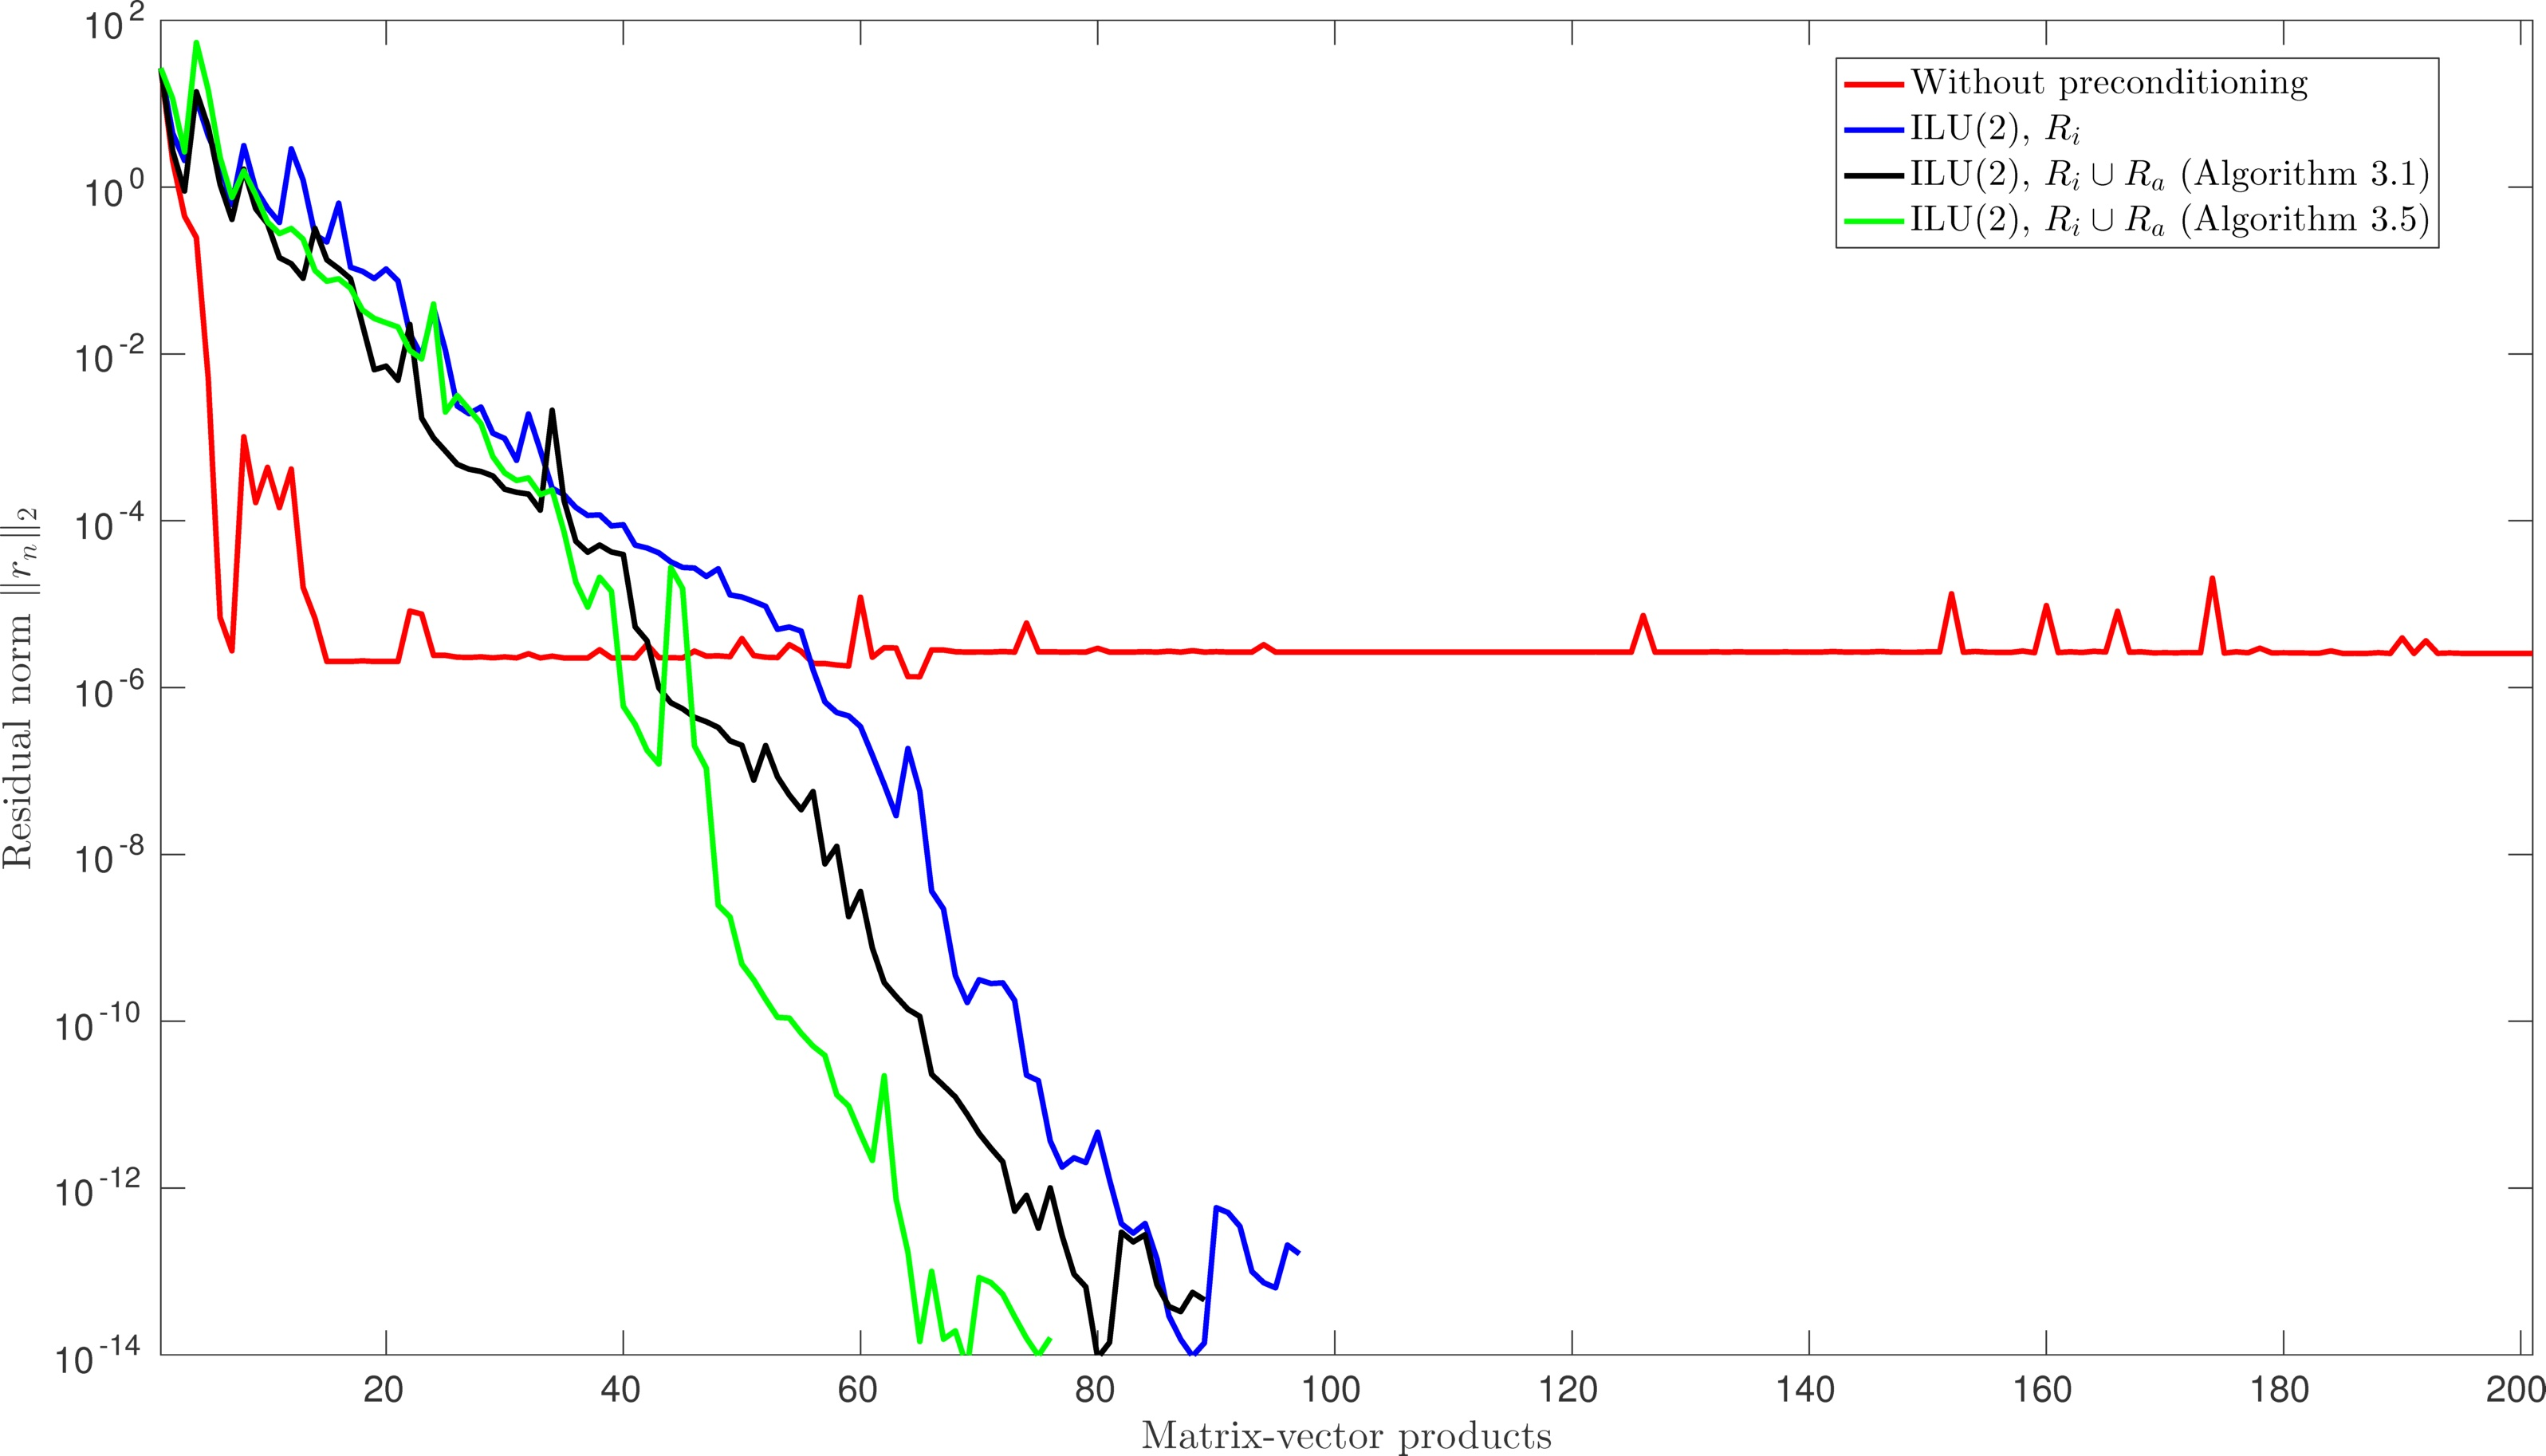
\includegraphics[width=0.9\textwidth]{jac_convergence_greedy_new_15}
\end{figure}
\end{frame}


\section{A Special Case}
\section{Conclusion}
\begin{frame}{Conclusion}
\begin{itemize}
\item Automatic Differenation and Preconditioning together
\item Using partial Jacobian Computation
\item Modeling in graph language
\item Some experimental results
\end{itemize}
\end{frame}

\begin{frame}{Finish!}
\begin{center}
   \Huge \bf Thank you!
\end{center}
\end{frame}

\end{document}

